\documentclass[review]{elsarticle}

\usepackage{lineno,hyperref}
\modulolinenumbers[5]

\journal{Journal of \LaTeX\ Templates}

%%%%%%%%%%%%%%%%%%%%%%%
%% Elsevier bibliography styles
%%%%%%%%%%%%%%%%%%%%%%%
%% To change the style, put a % in front of the second line of the current style and
%% remove the % from the second line of the style you would like to use.
%%%%%%%%%%%%%%%%%%%%%%%

%% Numbered
%\bibliographystyle{model1-num-names}

%% Numbered without titles
%\bibliographystyle{model1a-num-names}

%% Harvard
%\bibliographystyle{model2-names.bst}\biboptions{authoryear}

%% Vancouver numbered
%\usepackage{numcompress}\bibliographystyle{model3-num-names}

%% Vancouver name/year
%\usepackage{numcompress}\bibliographystyle{model4-names}\biboptions{authoryear}

%% APA style
%\bibliographystyle{model5-names}\biboptions{authoryear}

%% AMA style
%\usepackage{numcompress}\bibliographystyle{model6-num-names}

%% `Elsevier LaTeX' style
\bibliographystyle{elsarticle-num}
%%%%%%%%%%%%%%%%%%%%%%%


\usepackage[utf8]{inputenc}
\usepackage{amsmath}
\usepackage{amsfonts}
%\usepackage{textcomp}
\usepackage{graphicx}
%\usepackage{authblk}
\usepackage{subfig}
\usepackage{gensymb}

\graphicspath{{figs/}}

\begin{document}

\begin{frontmatter}

\title{Design of Space CoBot: an intra-vehicular astronaut assistant for space stations}
%\tnotetext[mytitlenote]{Fully documented templates are available in the elsarticle package on \href{http://www.ctan.org/tex-archive/macros/latex/contrib/elsarticle}{CTAN}.}

%% Group authors per affiliation:
\author{Pedro Roque}
\author[mycorrespondingauthor]{Rodrigo Ventura}
\address{Institute for Systems and Robotics \\
  Instituto Superior Técnico, Universidade de Lisboa \\
  Av. Rovisco Pais, 1, 1049-001 Lisboa, Portugal}
%\fntext[myfootnote]{Since 1880.}

%% or include affiliations in footnotes:
%\author[mymainaddress,mysecondaryaddress]{Elsevier Inc}
%\ead[url]{www.elsevier.com}

%\author[mysecondaryaddress]{Global Customer Service\corref{mycorrespondingauthor}}
\cortext[mycorrespondingauthor]{Corresponding author}
%\ead{support@elsevier.com}

%\address[mymainaddress]{1600 John F Kennedy Boulevard, Philadelphia}
%\address[mysecondaryaddress]{360 Park Avenue South, New York}

\begin{abstract}

  Collaborative robots, that is, robots that perform jointly and in interaction with humans some task, has been an active field of research for several years. However, this research has mostly focused on terrestrial domains. In this paper we address the problem of designing robot systems for collaborative tasks in space station environment. Space is a domain where most of the robotic applications are either fully automatic or fully teleoperated. For instance, there is almost no presence of autonomous mobile robots in the International Space Station (ISS).

  In this paper we address the problem of designing a fully autonomous mobile robot platform, called Space CoBot, for collaborative tasks with human astronauts inside a space station, as in the ISS. We assume microgravity and air ar atmospheric pressure. The proposed robot is fully holonomic, without any preferable direction of motion. The propulsion consists of 6 propellers driven by electric motors. The geometry of these propellers was obtained using a structural optimization approach, in order to balance thrust and torque across all directions. We then propose and validate in simulation a decoupled translational and attitude control scheme. Finally, we explore two proof-of-concept applications of the robot for a space station environment: debris scavenging, to clean up free flying small debris, and astronaut active motion stabilization. These two tasks are validated in a realistic simulator.

\end{abstract}

\begin{keyword}
Space robotics \sep Free flyer \sep International Space Station \sep collaborative robots \sep structural optimization
\end{keyword}

\end{frontmatter}

\linenumbers

% STRATEGY:
% - use SPACEBOTS SotA -- done
% - use IROS for vehicle design -- done
% - use UJCAI for tasks -- done
% - include Trey's feedback


\section{Introduction}
\label{sec:introduction}









\section{Vehicle design}
\label{sec:vehicle-design}


\subsection{Overall concept}
\label{sec:overall-concept}


% The Space CoBot is an approach to a microgravity UAV, capable of omnidirectional flying, to operate inside the International Space Station, as well as other microgravity atmosphered environments. In the development process, we selected the following guidelines: 
\begin{figure}
  \centering
  \subfloat[]{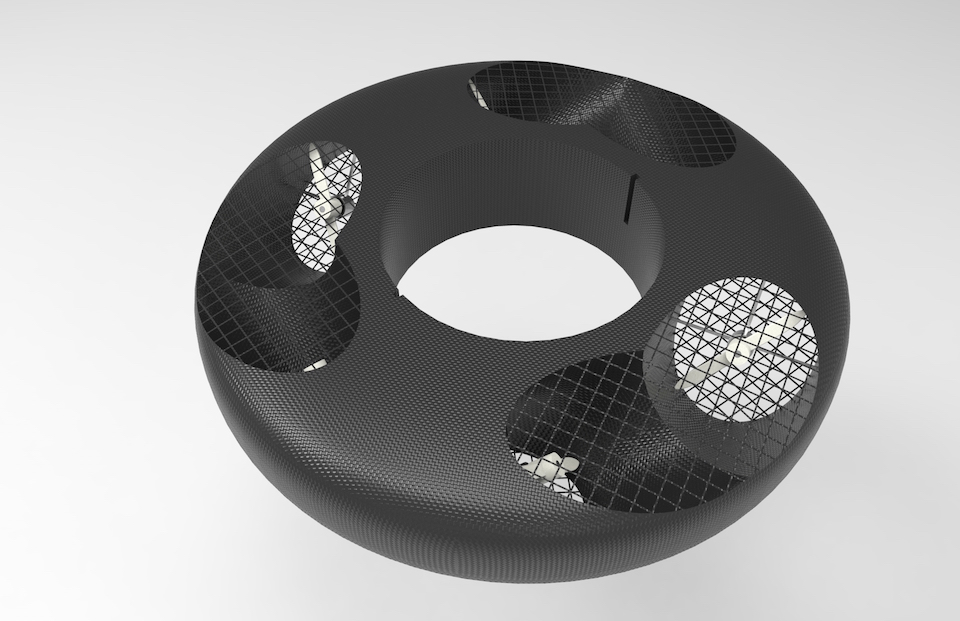
\includegraphics[width=0.49\linewidth]{propulsion_shell-smaller.jpeg}} \hfill
  \subfloat[]{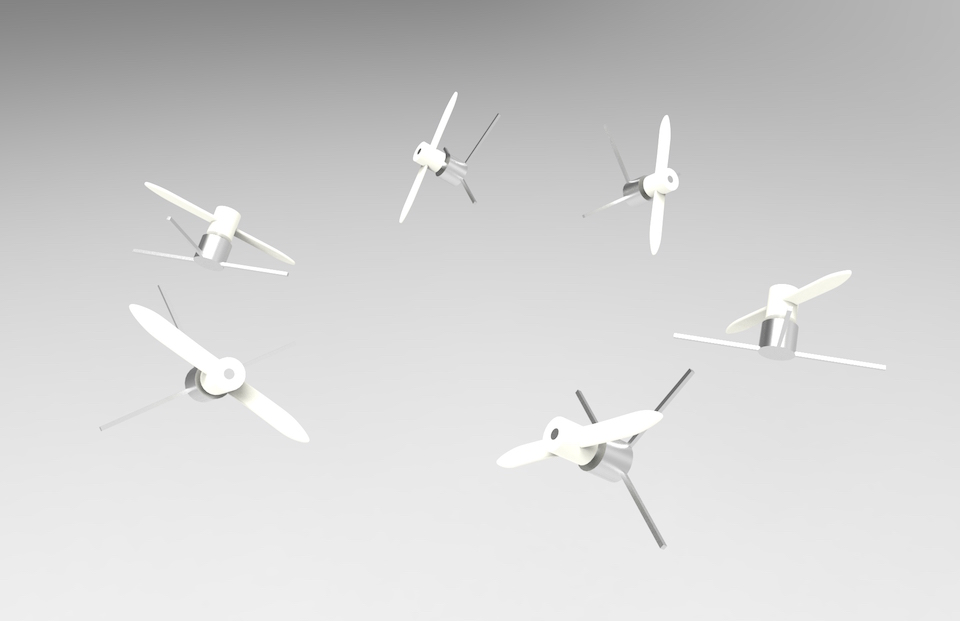
\includegraphics[width=0.49\linewidth]{propulsion_system-smaller.jpeg}}
  \caption{Propulsion system representation: (a)~overall view of the module, and (b)~relative placement of the propellers.}
  \label{fig:propulsion_system}
\end{figure}

% As starting point for the design of the aerial vehicle we considered
% the following requirements:
% \begin{enumerate}
% \itemsep=0em
% \item Safe operation;
% \item Self-contained and simple propulsion system, with holonomic
%   kinematics, that is, capable of motion in an arbitrary direction;
% \item Autonomous Guidance, Navigation and Control (GN\&C);
% \item Small dimensions;
% \item Modularity;
% \item Stackability and docking.
% \end{enumerate}

As space operation is expensive, we target a modular vehicle whose
parts can be easily maintained and that is easily extensible with
additional modules, e.g., hosting of scientific experiment
testbeds. An overview of all the modules is provided in Figure
\ref{fig:modules} and explained below.

\begin{figure}
  \centering
  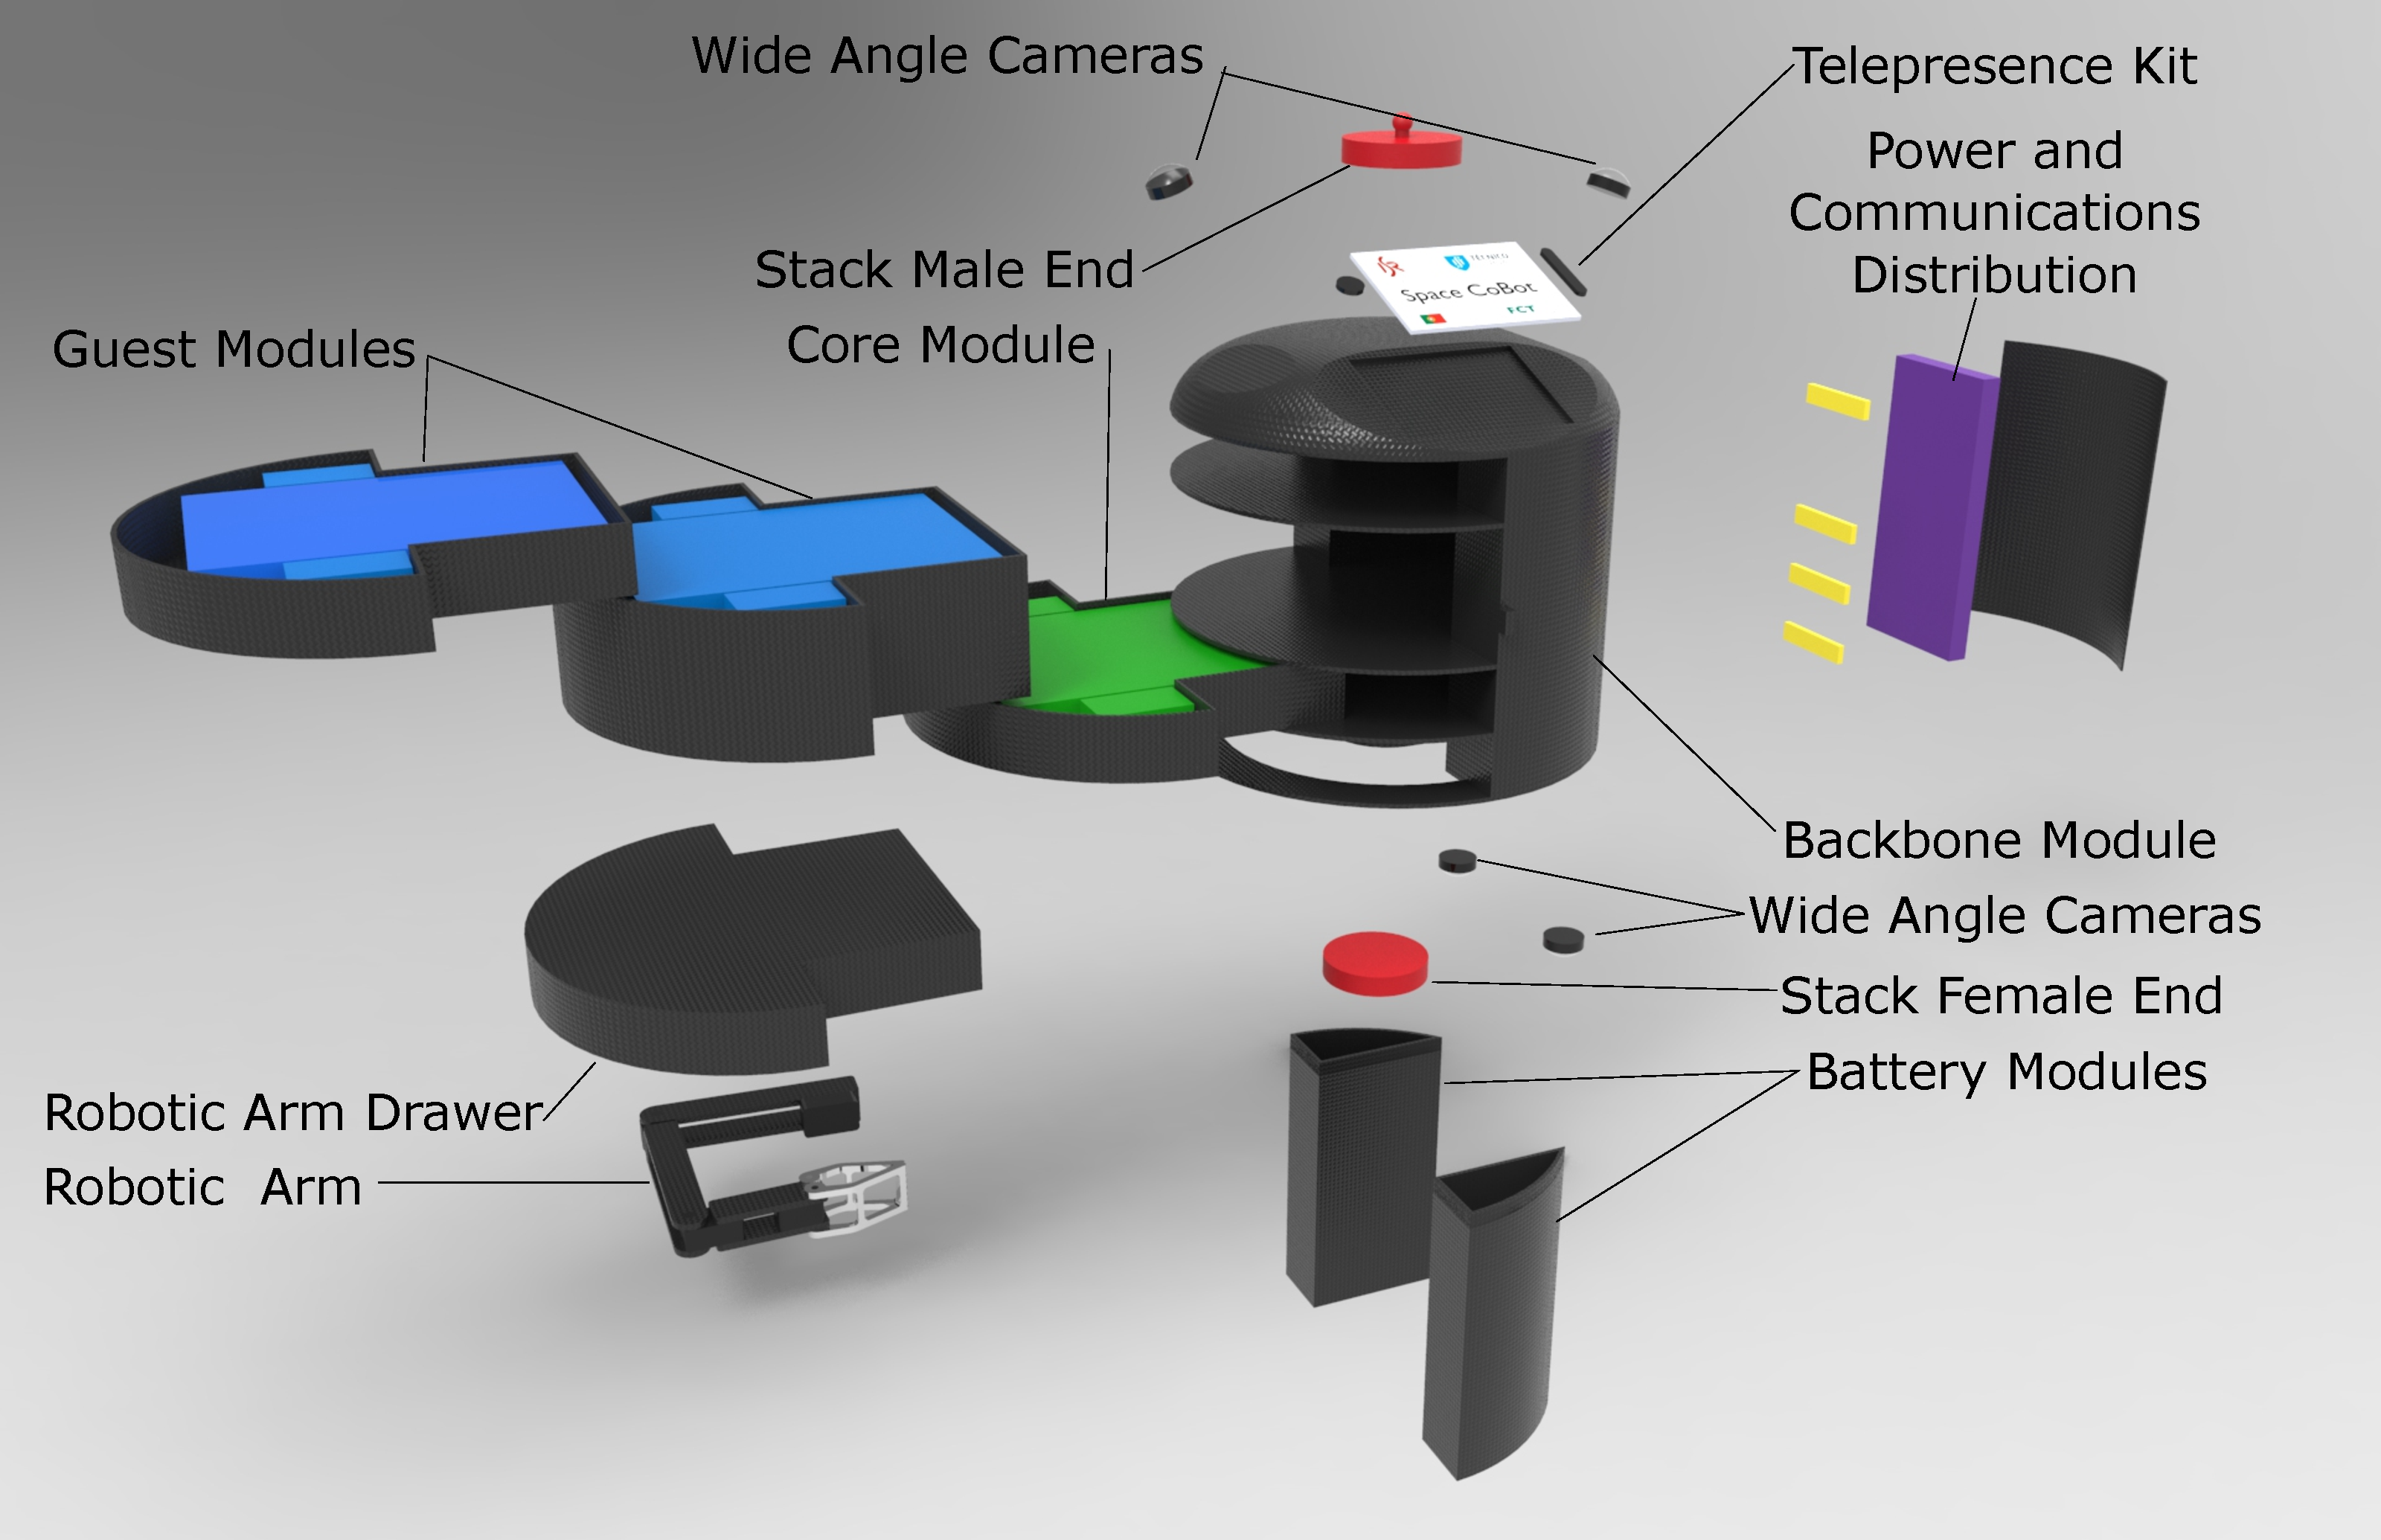
\includegraphics[width=0.95\linewidth]{new-explosion.pdf}
  \caption{Overall view of Space Cobot modules.}
  \label{fig:modules}
\end{figure}

To provide propulsion to the vehicle, we use 6 electric motors with
4'' propellers, arranged in such a way the kinematics is holonomic. We
defer a detailed description of this system, along with its
optimization, to Sections~\ref{sec:propulsion}
and~\ref{sec:design-parameters}. Our design of this system is shown in
Figure~\ref{fig:propulsion_system}.

The propulsion module attaches to the central core of the vehicle, a backbone module, that provides support for all remaining subsystems: batteries, a pair of docking connectors, cameras, extension modules, telepresence equipment, and a robotic manipulator.

For positioning inside the station we propose a vision-based
localization method employing 4 wide-angle cameras, two on the top
side of the vehicle and two on the bottom. These cameras also enable
visual servoing of the robotic arm. Autonomous navigation is
delivered by onboard computation, the Core module, capable of video
processing and propulsion actuation, as well the management of the
extension modules.

The docking ports provide multiple functions: they (1)~enable the
connection between the robot and a charging dock, they (2)~provide a
physical, solid connection between robots (stacking) for cooperative
tasks such as faster transportation of heavy loads. For charging, the
stacking of multiple robots also enables daisy-chained charging across several robots, thus saving space. A detailed view of the docking ports is provided on Figure~\ref{fig:coupling}.

\begin{figure}
  \centering
  \subfloat[]{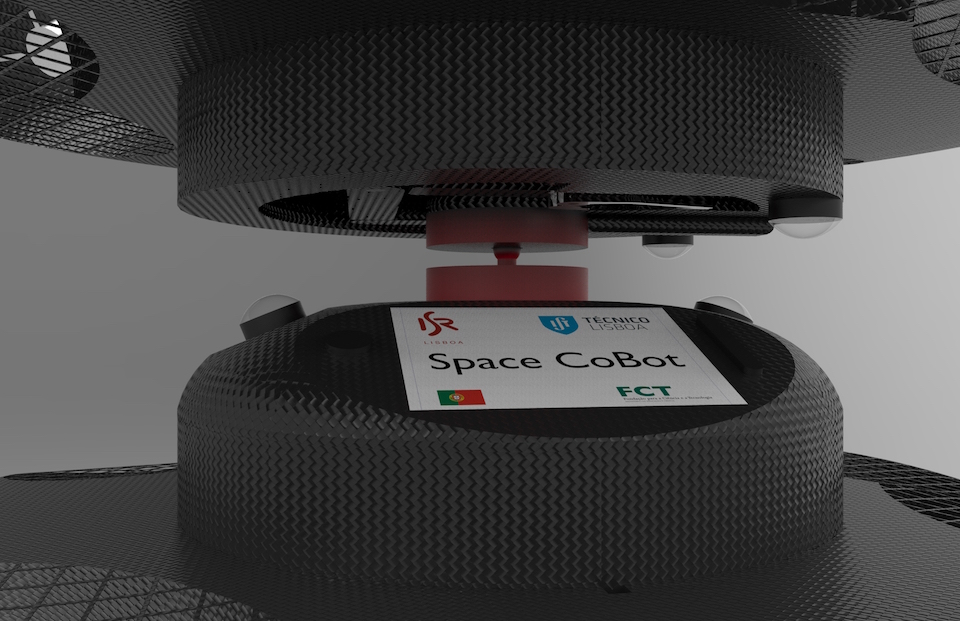
\includegraphics[width=0.49\linewidth]{coupling-detail-smaller.jpeg}} \hfill
  \subfloat[]{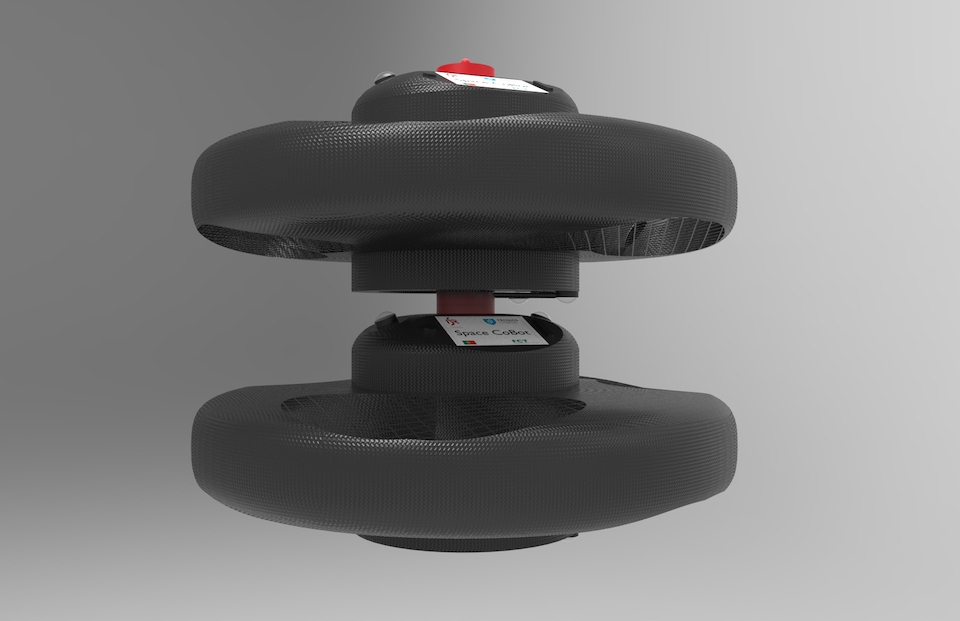
\includegraphics[width=0.49\linewidth]{coupling-view-smaller.jpeg}}
  \caption{Space Cobot coupling system : (a)~coupling mechanism detail , and (b)~two robots coupled together.}
  \label{fig:coupling}
\end{figure}

% Extension modules provide space testbeds for research centers. The robot can have a total of 2.4l of guest modules experiments that can range from control algorithms and electronics to fluid dynamics and small biological components. To access them, remote operation and monitoring of the robot is available, and also one can deploy such task on the Core module of the vehicle, for total autonomous experiment control. This results in a multipurpose testbed for space applications.

Two possible applications of the robot are telepresence and object
manipulation. Telepresence can be performed using the onboard display,
speakers, and microphone. Our design has enough space for a common
tablet-sized display. Mobile manipulation is crucial for robot-environment interaction. A robotic arm with a gripper is provided on the bottom part of the robot, providing several manipulation capabilities such as cargo transportation. This module fits in a standard module bay and can be replaced for additional guest module space.

For safer operation, electric propulsion was used instead of pressurized gas. Along with this, we also feature electromagnetic and acoustic noise reduction methods by using grounded copper mesh on the vehicles construction and acoustic absorvig materials around the motors airflow tunnel. With this, we aim at long periods of operation aboard space stations.


\subsection{Propulsion model}
\label{sec:propulsion-model}


% To derive the dynamical model of the vehicle, we start by modeling the
% force and torque vectors caused by a single propeller in the body
% frame denoted~$\mathcal{B}$, whose origin is coincident with the
% vehicle's center of mass (CoM).

% In this section we model the propulsion system, starting with the
% force and torque contributions to the vehicle body of single
% propeller, and then summing up the combining the contributions of them
% all.

Consider a single propeller $i$ whose motor is rigidly linked to the
body frame~$\mathcal{B}$, as depicted in Figure~\ref{fig:prop}.  This
propeller  generates a reaction force (thrust) $\bar{F}_i$ and  torque
$\bar{M}_i$ on the vehicle body.
While the former results directly from the
propeller thrust,
\begin{equation}
  \label{eq:Fi}
  \bar{F}_i = f_i \hat{u}_i \qquad %\quad\text{for}\quad
  f_i = K_1 u_i
\end{equation}
where $u_i$ is the actuation signal and $f_i$ is the scalar thrust,
the later is the sum of two components: the torque caused by the
non-central thrust
and the propeller reaction torque:
\begin{equation}
  \label{eq:Mi}
  \bar{M}_i = \bar{r}_i\times\bar{F}_i - \tau_i \hat{u}_i \qquad
  \tau_i = w_i K_2 u_i
\end{equation}
where $\times$ denotes vector cross product and $w_i$ is $-1$ or $1$
depending on whether the propeller rotates clockwise or anti-clockwise
for a positive forward thrust $f_i>0$.  These linear relationships
result from the momentum-blade element theory by considering $u=n^2$,
where $n$ is the blade's rotation speed (in revolutions per second) while the
constants $K_1$ and $K_2$ given by
\begin{equation}
  \label{eq:blade}
  K_1 = \rho D^4 C_T \qquad K_2 = \frac{\rho D^5}{2\pi} C_P
\end{equation}
where $\rho$ is the air density, $D$ is the propeller diameter, and
the $C_T$ and $C_P$ are blade dependent adimensional constants called
thrust and power coefficients~\cite{mccormick95}.

The relative position $\bar{r}_i$ of the $i$-th propeller, orthogonal to the
$Z$ axis, and the unit vector $\hat{u}_i$, aligned with the propeller
axis, are uniquely defined by the angles $\theta_i$ and $\phi_i$, and can be
easily obtained from geometrical reasoning by:
\begin{equation}
  \bar{r}_i = \left(
    \begin{array}{c}
      d\cos(\theta_i) \\
      d\sin(\theta_i) \\
      0
      \end{array}
    \right)
    \qquad
    \hat{u}_i = \left(
      \begin{array}{c}
        \sin(\theta_i)\sin(\phi_i) \\
        -\cos(\theta_i)\sin(\phi_i) \\
        \cos(\phi_i)
      \end{array}
      \right)
\end{equation}
where $d=\|\bar{r}_i\|$ is the distance from the propeller to the CoM.
Stacking together the resulting force $\bar{F}_i$ and torque
$\bar{M}_i$, one can obtain the linear relation
\begin{equation}
  \label{eq:fm}
  \left(
    \begin{array}{c}
      \bar{F}_i \\
      \bar{M}_i
    \end{array}
  \right) = \bar{a}_i\,u_i
\end{equation}
where
\begin{equation}
  \begin{split}
    \bar{a}_i  &= \left(
      \begin{array}{c}
        K_1 \hat{u}_i \\
        K_1 \bar{r}_i \times \hat{u}_i - w_i K_2 \hat{u}_i
      \end{array}
    \right) \\
    &= \left(
      \begin{array}{c}
        K_1 \sin(\theta_i)\sin(\phi_i) \\
        -K_1 \cos(\theta_i)\sin(\phi_i) \\
        K_1 \cos(\phi_i) \\
        \left[K_1 d \cos(\phi_i) - w_i K_2 \sin(\phi_i)\right]\sin(\theta_i) \\
        -\left[K_1 d \cos(\phi_i) - w_i K_2 \sin(\phi_i)\right]\cos(\theta_i) \\
        -K_1 d \sin(\phi_i) - w_i K_2 \cos(\phi_i)
      \end{array}
    \right)
    \end{split}
\end{equation}

\begin{figure}
  \centering
  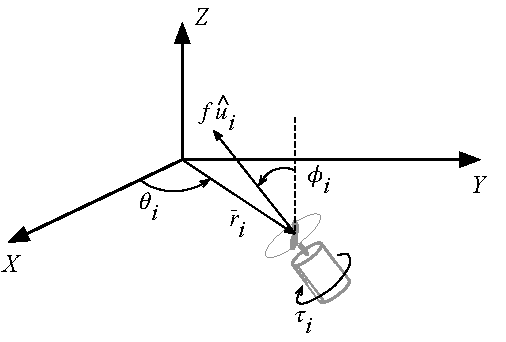
\includegraphics[width=0.6\linewidth]{prop.pdf}
  \caption{Notation used for modeling a single propeller with respect
    to the body frame~$\mathcal{B}$, centered on the vehicle's CoM.}
  \label{fig:prop}
\end{figure}

For a vehicle with $N$ propellers, the resulting force and torque will
be given by the sum of the contributions of each propeller, given with
respect to the CoM, by~\eqref{eq:fm}. This sum can be put in matrix
form as
\begin{equation}
  \label{eq:au}
  \left(
    \begin{array}{c}
      \bar{F} \\
      \bar{M}
    \end{array}
  \right) = \mathbf{A}\,\bar{u}
\end{equation}
where $\mathbf{A}=[\bar{a}_1 \cdots \bar{a}_N]$ is a square matrix,
hereby called \emph{actuation matrix}, and $\bar{u}=[u_1\cdots u_N]^T$
is the actuation input vector. \emph{The crucial observation is that, if the
actuation matrix $\mathbf{A}$ has at least rank 6, the linear
equation~\eqref{eq:au} can be solved for $\bar{u}$ for any given
combination of $\bar{F}$ and $\bar{M}$.}  A necessary (but not
sufficient\footnote{Sufficiency required $\mathbf{A}$ to be full
  rank.}) condition for this to be true is to have at least 6
propellers, thus justifying the hexarotor design considered in this
paper. Note that this matrix only depends on the vehicle's design
parameters, defined by the angles $\{\theta_i\}$ and $\{\phi_i\}$,
distance $d$, the trust coefficients $K_1$, $K_2$, and $\{w_i\}$.


\subsection{Structural optimization}
\label{sec:struct-optim}



In this section we will study how the design parameters translate to
the actuation matrix $\mathbf{A}$ defined in the previous section. In
particular, we will consider how actuation limits translates into
maximum values of force and torque. We will then optimize these
parameters in order to maximize the upper bound of forces and torques,
over all directions, imposed by a bounded actuation.

\subsubsection{Problem statement}
\label{sec:problem-statement}

% Throughout this paper we will assume that the propellers are equally
% distributed radially, that is,
% \begin{equation}
%   \label{eq:thetas}
%   \theta_i = (i-1) \frac{\pi}{3}
% \end{equation}
% For the sake of symmetry we will further consider the rotation
% directions to be alternating, that is,
% \begin{equation}
%   \label{eq:ws}
%   w_i =
%   \begin{cases}
%     1 & i\text{ is odd,} \\
%     -1 & i\text{ is even.}
%   \end{cases}
% \end{equation}

We will start by considering that each actuation signal is
bounded between $-1$ and $1$, that is,
\begin{equation}
  \label{eq:ahcube}
  -1 \leq u_i \leq 1 \quad \text{for} \quad i=1,\ldots,6
\end{equation}
According to \eqref{eq:au}, this hypercube will map onto a
6-dimensional convex polyhedron\footnote{A convex polyhedron is an
  intersection of a finite number of half-spaces~\cite{jeter86}.} in
the $(\bar{F}, \bar{M})$ space.  Any other choice of bounds is
possible by appropriately scaling constants $K_1$ and $K_2$.  However,
it assumes that the maximum propeller trust is symmetric with respect
to the direction of rotation~\footnote{Propellers may have different
thrust capabilities along each direction of the rotation axis. The
approach presented here can be easily extended to account for that asymmetry.}.
The remaining parameters are the angles
$\{\phi_i\}$. We will base our analysis on the optimization of these
angles with respect to various criteria.

Our goal will be to find the configurations of angles $\{\phi_i\}$
that maximize the range of forces (and torques) over all
directions.
% Conventional multirotors have all propellers directed at
% the same direction, \textit{i.e.,} with $\{\phi_i=0\}$,, which
% maximizes the thrust along that direction. However, they are unable to
% produce any thrust component over an orthogonal direction. By having
% nonzero values of $\{\phi_i\}$
% we expect to gain thrust over any direction, at the
% expense of reducing the maximum thrust over some particular one.
Geometrically, this corresponds to changing $\{\phi_i\}$
such that a ball of nonzero radius can fit inside the 3-dimensional
convex polyhedron in the $\bar{F}$ space mapped by the actuation
hypercube in~\eqref{eq:ahcube}, while keeping zero torque,
$\bar{M}=0$. A similar reasoning applies to the torque space
$\bar{M}$, while keeping $\bar{F}=0$. 
% In sum, we will look for the values of $\{\phi_i\}$ that
% maximize these radii.

First, we will address the problem of computing the maximum force
along a given direction specified as a unit vector $\hat{e}$, while
maintaining a zero torque.  From~\eqref{eq:au}, and assuming that
$\mathbf{A}$ is full rank, we get
\begin{equation}
  \bar{u} = \mathbf{A}^{-1}
  \left(
    \begin{array}{c}
      \bar{F} \\
      \bar{M}
    \end{array}
  \right) =\mathbf{A}^{-1}
  \left(
    \begin{array}{c}
      F \hat{e} \\
      0
    \end{array}
  \right)
\end{equation}
where $F>0$ is the force magnitude. For what follows, it will be
convenient to express the $\mathbf{A}^{-1}$ matrix as blocks of three
dimensional row vectors:
\begin{equation}
  \label{eq:bici}
  \mathbf{A}^{-1} = \left[
    \begin{array}{cc}
      b_1^T & c_1^T \\
      \vdots & \vdots \\
      b_6^T & c_6^T \\
    \end{array}
    \right]
\end{equation}
where $b_i,c_i\in\mathbb{R}^3$. Then, the actuation of the $i$-th
propeller is given by
\begin{equation}
  u_i = F b_i^T \hat{e}
\end{equation}
Since $|u_i|\leq1$, we have $F|b_i^T\hat{e}|\leq1$, and thus $F$ has
this upper bound:
\begin{equation}
  F \leq \frac{1}{|b_i^T\hat{e}|}
\end{equation}
Since this inequality has to be satisfied for all propellers
$i=1,\ldots,6$, the maximum force $F^\mathrm{max}_{\hat{e}}$ is given
by the lowest of these upper bounds
\begin{equation}
  F^\mathrm{max}_{\hat{e}} = \min_i \frac{1}{|b_i^T\hat{e}|}
\end{equation}
This force is the maximum force along a given direction $\hat{e}$. The
maximum force attainable in any direction can be obtained by
minimising this force over all possible directions. Since
$|b_i^T\hat{e}|\leq\|b_i\|$, this minimum is given by
\begin{equation}
  \label{eq:fmax}
  F^\mathrm{max} = \min_i \frac{1}{\|b_i\|}
\end{equation}
The same reasoning can be applied to the torques: consider a torque
$\bar{M}=M\hat{e}$ along an arbitrary direction defined by $\hat{e}$,
the corresponding actuation with $\bar{F}=0$ is $u_i=M c_i^T \hat{e}$,
resulting in the following maximum torque along any direction:
\begin{equation}
  \label{eq:mmax}
  M^\mathrm{max} = \min_i \frac{1}{\|c_i\|}
\end{equation}

Now, these maximum forces and torque values depend on the design
parameters. In the following we will use an optimization approach to
find the values of these parameters that maximize the maximum force
and/or torque. We will consider the propellers to be equally
distributed radially, that is,
\begin{equation}
  \label{eq:thetas}
  \theta_i = (i-1) \frac{\pi}{3}
\end{equation}
and a fixed distance $d$, as well as the constants $K_1$ and $K_2$. All the
remaining parameters will be the unknown variables:
\begin{equation}
  \bar{\psi} = ( \phi_1, \ldots, \phi_6, w_1,\ldots, w_6 )^T
\end{equation}
with the feasibility domain defined by
\begin{equation}
  \Psi = \left\{ \bar{\psi} \::\: |\phi_{1,\ldots,6}| \leq
  \phi_{max}, w_{1,\ldots,6}\in\{-1,1\} \right\}
\end{equation}
where $\phi_{max}$ is the maximum allowed deviation from the
vertical. As a mechanical constraint to allow obstructionless air flow
we considered $\phi_{max}=\pi/3$ in this work.

We can restate the maximization of~\eqref{eq:fmax}
and~\eqref{eq:mmax} using the epigraph form~\cite{boyd04}, thus getting rid of the
maximization of a minimum, in exchange of the introduction of two new
variables, $p$ and $q$:
\begin{equation}
  \label{eq:minp}
  \begin{split}
    &\text{minimize}\: p \\
    &\text{subject to:} \\
    &\quad p \geq \|b_i\|^2, i=1,\ldots,6
  \end{split}
\end{equation}
for the force and
\begin{equation}
  \label{eq:minq}
  \begin{split}
    &\text{minimize}\: q \\
    &\text{subject to:} \\
    &\quad q \geq \|c_i\|^2, i=1,\ldots,6
  \end{split}
\end{equation}
for the torque, where $\{b_i\}$ and $\{c_i\}$ depend non-linearly on
the parameters $\bar{\psi}$ through the inverse of the actuation
matrix $\mathbf{A}$ as~\eqref{eq:bici}. In this form, the optimization
variables are augmented with the cost, that is,
$\bar{\psi}_p=(p, \bar{\psi})$ for the problem~\eqref{eq:minp} and
$\bar{\psi}_q=(q, \bar{\psi})$ for~\eqref{eq:minq}.  It can be readily
seen that these forms maximize~\eqref{eq:fmax} and~\eqref{eq:mmax},
where the resulting maximum forces and torques can be recovered using
$F^{max}=1/\sqrt{p}$ and $M^{max}=1/\sqrt{q}$.

\subsubsection{Multi-criteria optimization}
\label{sec:multi-crit-optim}

The design optimization aims at maximizing simultaneously two
objective functions, force and torque ranges, given bounded
actuation~\eqref{eq:ahcube}. To do so we will take a multi-criteria
optimization approach~\cite{statnikov95}, combining the
optimization problems~\eqref{eq:minp}
and~\eqref{eq:minq} into a single multi-criteria problem:
\begin{equation}
  \label{eq:multi}
  \begin{split}
    &\text{minimize}\:(p, q) \\
    &\text{subject to:} \\
    &\quad p \geq \|b_i\|^2, i=1,\ldots,6 \\
    &\quad q \geq \|c_i\|^2, i=1,\ldots,6
  \end{split}
\end{equation}
In this problem, the optimization variables are augmented with both
$p$ and $q$, $\bar{\psi}_{pq}=(p, q, \bar{\psi})$, and we have two
cost functions, say $J_1(\bar{\psi}_{pq})=p$ and
$J_2(\bar{\psi}_{pq})=q$. The solution of this multi-criteria
optimization problem is the set $\mathcal{P}$ of non-dominated
solutions, defined by: $\bar{\psi}_{pq}^0\in P$ if and only if there is no
$\bar{\psi}_{pq}\in\Psi$ such that
$J_i(\bar{\psi})\leq J_i(\bar{\psi}^0)$ for all $i\in\{1,2\}$ and
$J_i(\bar{\psi})< J_i(\bar{\psi}^0)$ for at least one
$i\in\{1,2\}$. This set is also called \emph{Pareto optimal
  set}~\cite{statnikov95}, a subset of the \emph{objective space}
defined by all~$(J_1(\bar{\psi}),J_2(\bar{\psi}))$ for
$\bar{\psi}\in\Psi$.

Apart from very simple cases, the Pareto optimal set is not trivial to
obtain exactly. Thus, we will make a pointwise approximation using the
Normally Boundary Intersection (NBI) method~\cite{das98}. This method
is guaranteed to obtain Pareto optimal points if the objective space
is convex. But it is still capable of obtaining points in ``sufficiently
concave'' parts of the objective space~\cite{das98}.

The first step of NBI is to obtain the minimizers of the each cost
function taken individually. These are also called \emph{shadow
  minima}. Let us start by considering the first minimization
problem~\eqref{eq:minp}, where $\bar{\psi}^*_p$ is the minimizer with
minimum cost $p^*$.  Then, this minimizer both minimizes $p$
in~\eqref{eq:multi} and, together with $q^0=\max_i\,\|c_i\|^2$, is a
non-dominated solution of~\eqref{eq:multi}, and thus belongs to its
Pareto optimal set. This results from the fact that this $q^0$ is the
smallest one that still satisfies the constrains of~\eqref{eq:multi}:
any $(p^*,q)$ with $q>q^0$ is dominated by $(p^*,q^0)$.  The same
reasoning can be applied to~\eqref{eq:minq}, resulting in the
minimizer $\bar{\psi}^*_q$, with minimum cost $q^*$, that together
with $p^0=\max_i\,\|b_i\|^2$ is also a non-dominated solution
of~\eqref{eq:multi}, thus also belonging to its Pareto optimal set.

On the $(p,q)$ space, these two non-dominated solutions corresponds
to two extremal points, $(p^*,q^0)$ and $(p^0,q^*)$, of the Pareto
optimal set: no feasible solutions exists neither to the left of
$p^*$ nor lower than $q^*$. \emph{The application of NBI to a two cost
function problem amounts to scanning along a straight line joining
$(p^*,q^0)$ and $(p^0,q^*)$, and then, for each point on this
straight line, to determine the single non-dominated solution along
the orthogonal direction.}

\begin{figure}
  \centering
  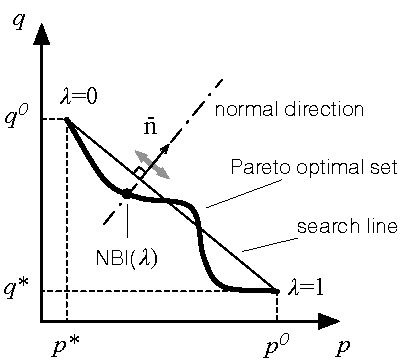
\includegraphics[width=0.6\linewidth]{nbi.pdf}
  \caption{Illustration of the NBI method: given a point defined by
    $\lambda\in[0;1]$, along the search line between $(p^*,q^0)$ and
    $(p^0,q^*)$, the optimization is done along the normal direction
    spawned by vector $\bar{n}$, resulting on the $NBI(\lambda)$
    intersection point.}
  \label{fig:nbi}
\end{figure}

Figure~\ref{fig:nbi} illustrates the NBI method. This straight line
can be parametrized by a $\lambda$ value ranging between 0 and 1,
resulting in $(1-\lambda)(p^*,q^0)+\lambda\,(p^0,q^*)$. An
orthogonal direction to this straight line is spawned by the vector
$\bar{n}=(q^0-q^*,p^0-p^*)$. Using again the epigraph form, but now
along this vector, we obtain the following constrained optimization
problem:
\begin{equation}
  \label{eq:nbi}
  \begin{aligned}
    &\text{minimize}\: t \\
    &\text{subject to:} \\
    &\quad (q^0-q^*)\,t + (1-\lambda) p^* + \lambda p^0 &\geq
    \|b_i\|^2 \\
    &\quad (p^0-p^*)\,t + \lambda q^* + (1-\lambda) q^0 &\geq
    \|c_i\|^2 \\
    &\qquad \text{for } i=1,\ldots,6
  \end{aligned}
\end{equation}
with the augmented vector $\bar{\psi}_t=(t, \bar{\psi})$ as
optimization variable. For a given $\lambda\in[0;1]$, the solution of
this optimization problem yields a minimizer $\bar{\psi}^*_t(\lambda)$
from which the corresponding point in the $(p,q)$ space is
\begin{equation}
  NBI(\lambda) = (p_\lambda, p_\lambda), \quad p_\lambda = \min_i \|b_i\|^2, \quad q_\lambda = \min_i \|c_i\|^2
\end{equation}
from which the maximum values of force and torque can be recovered as
above mentioned.

Since these problems cannot be solved in closed form, we will make use
of numerical optimization methods. The following section presents the
numerical results obtained for this problem.


% Considering the angles $\{\phi_i\}$ as the only design
% parameters, the following optimization problem can be formulated:
% \begin{equation}
%   \Phi^* = \min_{\Phi\in\mathcal{P}} J(\Phi)
% \end{equation}
% where $J$ is the cost function, $\Phi=[\phi_1\cdots\phi_6]^T$, and $\mathcal{P}$ is the set of
% allowable angle values. As cost function we consider a linear
% combination of the symmetric of the maximum force and torque,
% \begin{equation}
%   J(\Phi) = -(1-\lambda) F^\mathrm{max} - \lambda M^\mathrm{max}
% \end{equation}
% which corresponds to a linear scalarization of a multi-objective
% problem consisting of the objective functions~\eqref{eq:fmax}
% and~\eqref{eq:mmax}.  This problem is neither convex, smooth, not
% linear, so we will employ global optimization methods to solve it
% numerically. In particular, the results presented below were obtained
% using differential evolution algorithm~\cite{storn97}.

% Recall that the values of parameters $\{\theta_i\}$ and $\{w_i\}$ are
% set according to \eqref{eq:thetas} and \eqref{eq:ws}. For the
% $\{\phi_i\}$ we will consider three cases:
% \begin{enumerate}
% \item the simplest one consists in alternating a single angle value between
%   two symmetric values, similarly to what is done in~\cite{jiang13,voyles12}, that is
%   \begin{equation}
%     % \mathcal{P}_1 = \left\{ (\phi, -\phi, \phi, -\phi, \phi, -\phi)^T \::\:
%     %   \phi\in[0; \frac{\pi}{2}] \right\}
%     \mathcal{P}_1 = \left\{ \left(
%         \begin{array}{r}
%           \phi \\ -\phi \\ \phi \\ -\phi \\ \phi \\ -\phi
%         \end{array}
%       \right) \::\: |\phi|<\frac{\pi}{2}] \right\}
%   \end{equation}
% \item next we consider three degrees of freedom, corresponding to the
%   three principal axes joining pair os motors at opposite sides, that
%   is
%   \begin{equation}
%     % \mathcal{P}_3 = \left\{ (\phi_1, \phi_2, \phi_3, -\phi_1, -\phi_2, -\phi_3)^T \::\:
%     %   \phi_1\in[0; \frac{\pi}{2}], \phi_2,\phi_3\in[0; \frac{\pi}{2}] \right\}
%     \mathcal{P}_3 = \left\{ \left(
%         \begin{array}{r}
%           \phi_1 \\ \phi_2 \\ \phi_3 \\ -\phi_1 \\ -\phi_2 \\ -\phi_3
%         \end{array}
%       \right) \::\: |\phi_{1,\ldots,3}|<\frac{\pi}{2} \right\}
%   \end{equation}
% \item finally, there is the case where we have the six degrees of
%   freedom, one for each propeller, that
%   is
%   \begin{equation}
%     % \mathcal{P}_3 = \left\{ (\phi_1, \phi_2, \phi_3, -\phi_1, -\phi_2, -\phi_3)^T \::\:
%     %   \phi_1\in[0; \frac{\pi}{2}], \phi_2,\phi_3\in[0; \frac{\pi}{2}] \right\}
%     \mathcal{P}_3 = \left\{ \left(
%         \begin{array}{r}
%           \phi_1 \\ \phi_2 \\ \phi_3 \\ \phi_4 \\ \phi_5 \\ \phi_6
%         \end{array}
%       \right) \::\: |\phi_{1,\ldots,6}|<\frac{\pi}{2} \right\}
%   \end{equation}
% \end{enumerate}
% We have considered an unilateral interval for one of the propellers
% for symmetry breaking, since inverting the signs of all the $\phi_i$
% angles would result in the same cost function values.

\subsubsection{Numerical results}
\label{sec:numerical-results}

The optimization problem in~\eqref{eq:nbi} shows some features that
make it non-trivial to solve: it is both strongly non-convex with
mixed continuous and discrete variables. First, we will factor out the
discrete part by iteratively trying each combination of $\{w_i\}$
values modulo rotations (also called \emph{orbits}\footnote{For
  instance, $[1,-1,1,1,1,1]$ and $[1,1,-1,1,1,1]$ belong to the same
  orbit, and thus it is redundant to try both of them.}): from its
$2^6=64$ possible combinations, only 14 correspond to combinations
where no pair can be made equal after rotating one of them. Second, we
use a random multistart initialization together with a convex
optimization algorithm: for each sample drawn uniformly from the
$\{\phi_i\::\:|\phi_i| \leq \phi_{max}\}$ cube, we run the Constrained
Optimization BY Linear Approximation (COBYLA) algorithm~\cite{powell94},
as implemented in the SciPy optimization package.

% - explicar valores de K

To make the relation between force and actuation dimensionless, we
divided the actuation matrix by $K_1$. This way, the only dependence
on physical coefficients of this matrix is on the parameters $d$ and
the ratio $K_2/K_1$. Using~\eqref{eq:blade}, this ratio can be
expressed as
\begin{equation}
  \frac{K_2}{K_1} = \frac{D}{2\pi} \frac{C_P}{C_T}
\end{equation}
For various small propellers (of about 4'') we found\footnote{We used the
  UIUC Propeller Data Site, Vol. 2,
  http://m-selig.ae.illinois.edu/props/propDB.html (retrieved
  Nov-2015).} this ratio to be approximately~0.01. And thus we used
this value to obtain the numerical results presented in this section.
For $d$ we used the one from the design presented in
Section~\ref{sec:vehicle-design}, that is, $d=0.16$.

% - mostrar shadow optima

The extremes of the NBI search line are the shadow minima,
\textit{i.e.,} the minima of~\eqref{eq:minp}
and~\eqref{eq:minq}. For~1000 random initializations, we obtained
these values for the shadow minima: $(p^*,q^0)=(0.250, 15.01)$ and
$(p^0,q^*)=(0.4167,9.728)$.

% - mostrar resultados NBI

\begin{figure*}
  \centering
  \subfloat[]{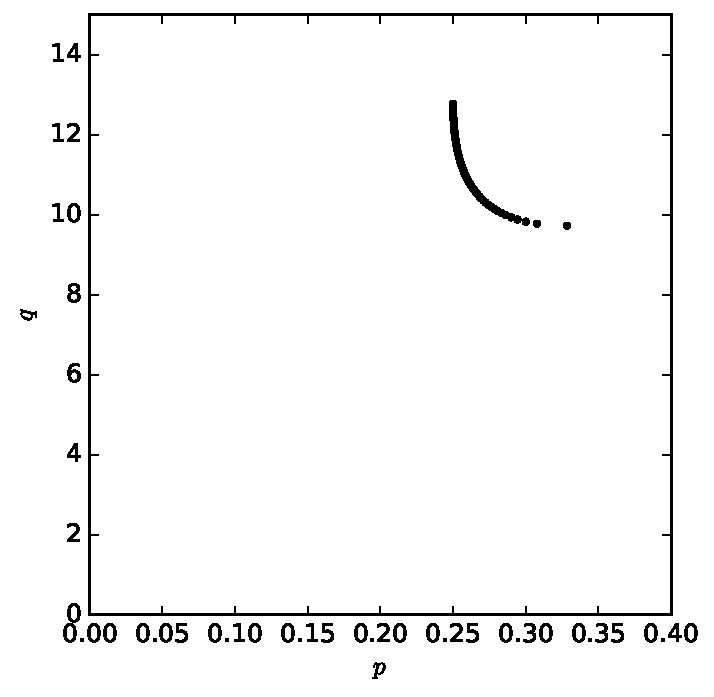
\includegraphics[height=0.28\linewidth]{nbi_pq.pdf}} \hfill
  \subfloat[]{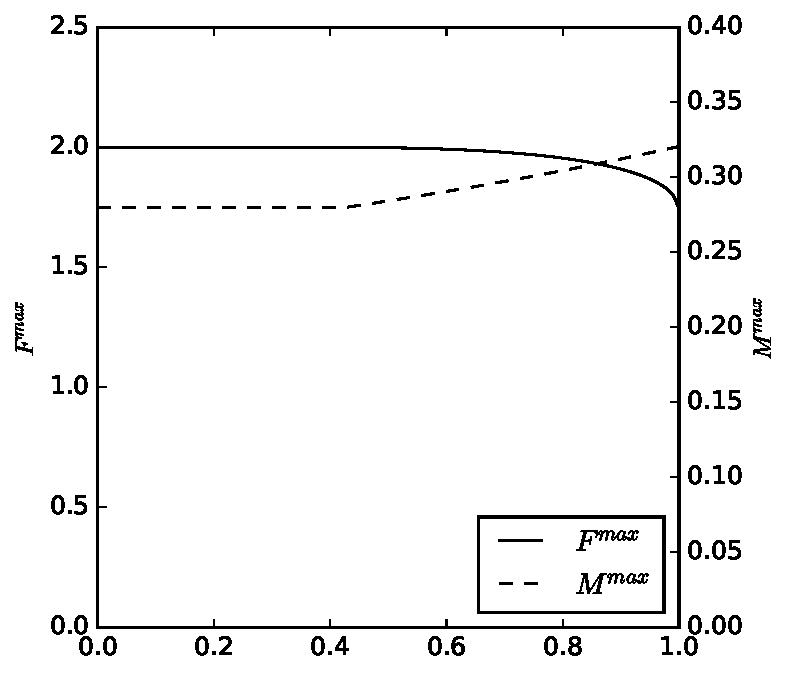
\includegraphics[height=0.28\linewidth]{nbi_fml.pdf}} \hfill
  \subfloat[]{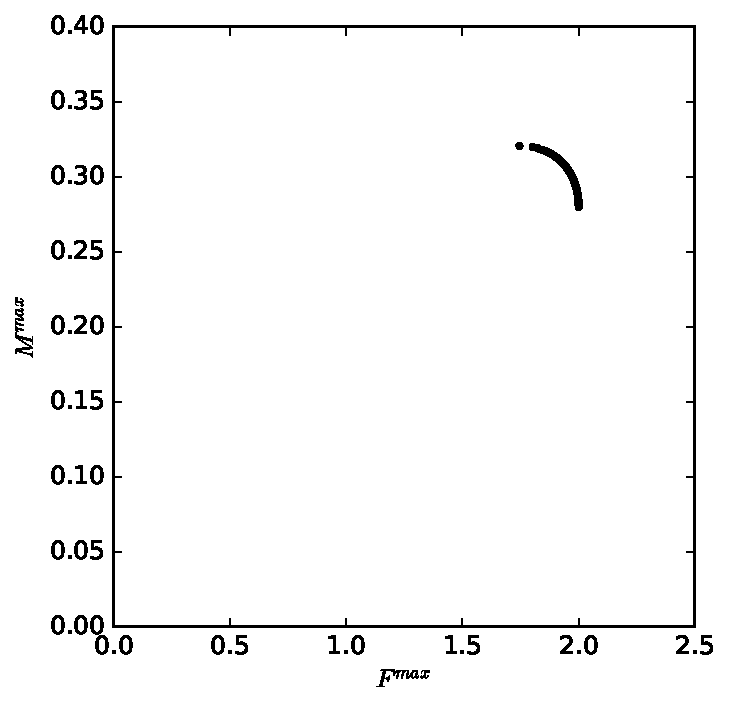
\includegraphics[height=0.28\linewidth]{nbi_FM.pdf}}
  \caption{Pointwise approximation to the Pareto optimal set using the
    NBI method: (a)~obtained points in the $(p.q)$ space,
    (b)~$F^{max}$ and $M^{max}$ in function of $\lambda$, and (c)~in
    the $(F^{max},M^{max})$ space. The dimensions for $F^{max}$ and
    $M^{max}$ have no physical meaning because of the division of the
    actuation matrix by~$K_1$, as explained in the text, and thus are
    to be understood in relative terms only.}
  \label{fig:nbiout2}
\end{figure*}

\begin{table*}
  \centering
  \begin{tabular}{l|cccccc|rrrrrr|cc}
    $\lambda$
    & $\phi_1$ & $\phi_2$ & $\phi_3$ & $\phi_4$ & $\phi_5$ & $\phi_6$
    & $w_1$ & $w_2$ & $w_3$ & $w_4$ & $w_5$ & $w_6$
    & $F^{max}$ & $M^{max}$ \\
    \hline
    0
    & 54.74 &-54.73 & 54.74 &-54.74 & 54.73 &-54.74
    &-1 & 1 &-1 & 1 &-1 & 1
    & 2.000 & 0.2798 \\
    0.25
    & 54.73 &-54.74 & 54.74 &-54.73  & 54.74 &-54.74
    &-1 & 1 &-1 & 1 &-1 & 1
    & 2.000 & 0.2798 \\
    0.5
    & 53.73 &-53.73 & 53.73 &-53.73 & 53.73 &-53.73
    &-1 & 1 &-1 & 1 &-1 & 1
    & 1.999 & 0.2844 \\
    0.75
    & 49.56 &-49.56 & 49.56 &-49.56 & 49.56 &-49.56
    &-1 & 1 &-1 & 1 &-1 & 1
    & 1.969 & 0.3009 \\
    1
    & 38.84 &-38.85 & 38.84 &-38.84  & 38.85 &-38.84
    &-1 & 1 &-1 & 1 &-1 & 1
    & 1.745 & 0.3206 \\
    \hline
  \end{tabular}
  \caption{Some of the configurations obtained for 5 equally spaced
    values of $\lambda$. The values for $\{\phi_i\}$ are shown in
    degrees. As before, the dimensions for $F^{max}$ and
    $M^{max}$ have no physical meaning.}
  \label{tab:configs}
\end{table*}

With these values, we ran our optimization method for $\lambda$
ranging from~0 to~1 on 0.01 steps, for 1000 random initializations
each. The result is a set of points approximating the Pareto optimal
set, shown in Figure~\ref{fig:nbiout2}. The (a) plot of this figure
suggests a convex Pareto front. For a range of $\lambda$ values from 0
to about 0.4, the $(p,q)$ values are constant. As $\lambda$ increases
over 0.4, there is a drop on the values of $q$, meaning a slight
increase on $M^{max}$

% - justificar escolha

\begin{table}
  \centering
  \begin{tabular}{ccccccc}
    propeller ($i$) & 1 & 2 & 3 & 4 & 5 & 6 \\
    \hline
    $\theta_i$ & 0 & 60 & 120 & 180 & 240 & 300 \\
    $\phi_i$ & 55 & -55 & 55 & -55 & 55 & -55 \\
    $w_i$ & -1 & 1 & -1 & 1 & -1 & 1 \\
    \hline
  \end{tabular}
  \caption{Design parameters of the selected solution. Both
    $\{\theta_i\}$ and $\{\phi_i\}$ are expressed in degrees.}
  \label{tab:selected}
\end{table}

Table~\ref{tab:configs} shows some of the optimal configurations
obtained for some values of $\lambda$. In our choice we decided to
prefer maximum force,
since the corresponding maximum torque is not significantly
lower than other non-dominated solutions, and thus we selected a configuration found in
the lower range of $\lambda$ values. We rounded off the angle values
to the closest integer degree, resulting in the configuration shown in
Table~\ref{tab:selected}. All of the following results shown in this
paper employ this selected configuration.




% We applied this methodology to a vehicle with the design parameters
% shown in Table~\ref{tab:params}. The constants $K_1$ and $K_2$ have
% the same values than the ones reported in \cite{jiang13msc}, while $d$
% is the one from the design presented in
% Section~\ref{sec:specification}.

% \begin{table}
%   \centering
%   \begin{tabular}{ccccc}
%     $K_1$ & $K_2$ & $d$ & $\{\theta_i\}$  \\
%     \hline
%     5.7 & 1.3 & 0.16 & in \eqref{eq:thetas}  \\
%   \end{tabular}
%   \caption{Design parameters of the simulated vehicle.}
%   \label{tab:params}
% \end{table}

% To get an idea of the shape of the feasible set in the space of costs
% values, we sampled $N$ points uniformly from $\Psi$ and identified the
% non-dominated points. The result is shown in
% Figure~\ref{fig:pareto}. Although these non-dominated points are an
% unstable approximate to the Pareto optimal set, they suggest that a
% linear scalarization of the cost functions should provide a good
% approximation to the actual Pareto optimal set.

% \begin{figure}
%   \centering
%   
\includegraphics[width=0.8\linewidth]{pareto_12.png}
%   \caption{Samples ($N=10^7$) uniformly drawn from the feasible set $\Psi$ shown
%     in the cost functions space. The non-dominated samples are shown
%     as bigger points.}
%   \label{fig:pareto}
% \end{figure}

% The shadow minimum is defined by the optimization of the individual
% cost functions, that is,
% \begin{equation}
%   J_1^* = \min_{\bar{\psi}} J_1(\bar{\psi}) \qquad
%   J_2^* = \min_{\bar{\psi}} J_2(\bar{\psi})
% \end{equation}
% After running differential evolution over~100 runs, we obtained the
% minimum values $J_1^*=-11.40$ and $J_2^*=-3.176$ (with a total variation
% below~$10^{-3}$).

% % The shadow minimum is defined by the optimization of the individual
% % cost functions, that is,
% % \begin{equation}
% %   \bar{\psi_1^*} = \argmin_{\bar{\psi}} J_1(\bar{\psi}) \qquad
% %   \bar{\psi_2^*} = \argmin_{\bar{\psi}} J_2(\bar{\psi})
% % \end{equation}
% % These minimizers corresponds to two points in the costs function
% % space, say $(J_1^*,J_2^+)=( J_1(\bar{\psi_1^*}),J_2(\bar{\psi_1^*}))$
% % and $(J_1^+,J_2^*)=( J_1(\bar{\psi_2^*}),J_2(\bar{\psi_2^*}))$. The
% % line between these two points is called the \emph{convex hull of
% %   individual minima} (CHIM)}. If the Pareto optimal set is convex,
% % which from Figure~\ref{fig:pareto} seems to be the case, then it
% % certainly lies below the CHIM line~\cite{das98}. After running
% % differential evolution over~100 runs, we obtained the mean values
% % $(J_1^*,J_2^+)=(-11.40, -2.606)$ and
% % $(J_1^+,J_2^*)=(-9.260 , -3.176)$.

% We applied the linear scalarization~\eqref{eq:linscal} and used a
% differential evolution\footnote{We used the implementation found in
%   the \emph{optimize} package of SciPy. We used the default parameters
%   except for a population size of 512 and a mutation dithering range
%   of~$[0.2; 0.6]$.} algorithm~\cite{storn97} on this cost function,
% while ranging $\lambda$ over an equally spaced grid from 0 to 1
% totalling 20 runs. Figure~\ref{fig:pm12} shows the obtained
% results. The bottom left solution in the \ref{fig:pm12}(b) plot, which
% approximately dominates all of the others, includes 12 of these 20
% runs. 

%  \begin{figure}
%   \centering
%   % data from rm12dep_2.npy
%   \subfloat[]{
\includegraphics[width=0.33\linewidth]{out_pm12_cost.pdf}}
%   \subfloat[]{
\includegraphics[width=0.33\linewidth]{out_pm12_pareto.pdf}}
%   \subfloat[]{
\includegraphics[width=0.33\linewidth]{out_pm12_solution.pdf}}
%   \caption{Optimization results,
%     from left to right: (a)~plot of $J$, $J_1=-F^\mathrm{max}$, and
%     $J_2=M^\mathrm{max}$ in function of $\lambda$, (b)~solutions found
%     shown in the $J_1$ and $J_2$ space, and (c)~optimized $\{\phi_i\}$
%     in function of~$\lambda$.}
%   \label{fig:pm12}
% \end{figure}

% We then ran differential evolution 100 times with
% $\lambda=0.4$, an heuristically chosen within a range of $\lambda$
% values where the resulting costs seem stable. From these runs, the
% dominant solution, found in 24 of these 100 runs, is shown in
% Table~\ref{tab:best}. Its costs are $J_1=-11.40$ and $J_2=-3.176$,
% which coincide with the individual minima $J_1^*$ and $J_2^*$ found
% above. That is, no other solution found has lower cost in either of
% the cost functions. 

% \begin{table}
%   \centering
%   \begin{tabular}{ccccccc}
%     propeller ($i$) & 1 & 2 & 3 & 4 & 5 & 6 \\
%     \hline
%     $\theta_i$ & 0\textdegree & 60\textdegree & 120\textdegree & 180\textdegree & 240\textdegree & 300\textdegree \\
%     $\phi_i$ & -74.54\textdegree & -39.54\textdegree & -74.57\textdegree & -39.48\textdegree & -74.49 \textdegree & -39.46 \\
%     $w_i$ & -1 & 1 & -1 & 1 & -1 & 1 \\
%     \hline
%   \end{tabular}
%   \caption{The solution found over 100 runs of the optimizer with
%     $\lambda=0.4$.}
%   \label{tab:best}
% \end{table}

% To wrap up these results, Figure~\ref{fig:costs} shows the solutions
% found by differential evolution as boxplots, in three different
% scenarios: the solutions for the two shadow minima
% $\bar{\psi}_1^*=\arg\min J_1(\bar{\psi})$ and
% $\bar{\psi}_2^*=\arg\min J_2(\bar{\psi})$, and the solutions
% $\bar{\psi}_\lambda^*=\arg\min J(\bar{\psi}; \lambda)$ for
% $\lambda=0.4$. Note that the minimum costs of the
% $\bar{\psi}_\lambda^*$ solutions coincide with the individual
% minima of $J_1^*=J_1(\bar{\psi}_1^*)$ and $J_2^*=J_2(\bar{\psi}_2^*)$.

% \begin{figure}
%   \centering
%   
\includegraphics[width=0.8\linewidth]{out_osom12.pdf}
%   \caption{Boxplots of the $J_1$ and $J_2$ costs found while
%     separately minimizing, $J_1(\bar{\psi})$ (first and second
%     boxplot), $J_2(\bar{\psi})$ (third and fourth boxplot), and
%     $J(\bar{\psi}; \lambda)$ for $\lambda=0.4$ (fifth and
%     sixth). Each boxplots represents the minimum, maximum, and median
%     values.}
%   \label{fig:costs}
% \end{figure}

% The solution in Table~\ref{tab:best} implies three of the propellers to be
% almost horizontal, hindering the air flow to produce the desired
% thrust. Therefore, we decided on a different solution, with the angle
% values rounded from an handpicked solution from the Pareto optimal set
% obtained above. Its parameters are shown in Table~\ref{tab:selected}
% and its costs are $J_1=-F^\mathrm{max}=-11.40$ and
% $J_2=-M^\mathrm{max}=-2.623$, that is, the same maximum force but with
% 82\% of the maximum torque. We preferred this solution
% because the propeller angles are not as horizontal, resulting in a
% significantly better air flow.
% % Running the
% % optimization algorithm on a restricted feasibility space parametrized
% % by~$\phi$ defined as
% % \begin{equation}
% %   \bar{\psi} = \left(-\phi, \phi, -\phi, \phi, -\phi, \phi, -1, -1, 1, 1,
% %     1, -1\right)^T
% % \end{equation}
% % with $\lambda=0.4$ resulted 

% \begin{table}
%   \centering
%   \begin{tabular}{ccccccc}
%     propeller ($i$) & 1 & 2 & 3 & 4 & 5 & 6 \\
%     \hline
%     $\theta_i$ & 0\textdegree & 60\textdegree & 120\textdegree & 180\textdegree & 240\textdegree & 300\textdegree \\
%     $\phi_i$ & -55\textdegree & 55\textdegree & -55\textdegree & 55\textdegree & -55\textdegree & 55\textdegree \\
%     $w_i$ & -1 & -1 & 1 & 1 & 1 & -1 \\
%     \hline
%   \end{tabular}
%   \caption{Design parameters of the selected solution.}
%   \label{tab:selected}
% \end{table}


% Figure~\ref{fig:forces} shows the maximum forces and torques in set
% $\mathcal{P}_1$. The cost functions~\eqref{eq:fmax}
% and~\eqref{eq:mmax} correspond to the symmetric of the pointwise
% minimum over the three lines for each one of these plots. The
% non-convexity of the cost functions is clearly visible in this plot. When
% $\phi=0$ the maximum force is zero, since in this configuration all
% thrust is directed along the $Z$ axis: this corresponds to the
% usual configuration of hexacopters (and quadrotors, although with less
% propellers). As $|\phi|$ increases, the maximum force along directions
% other than $Z$ increases.

% \begin{figure}
%   \centering
%   
\includegraphics[width=\linewidth]{out_plot_forces.pdf}
%   \caption{Maximum force and torque, $F^\mathrm{max}$ and
%     $M^\mathrm{max}$, for each one of
%     the body frame axes while ranging across the design space
%     $\mathcal{P}_1$.}
%   \label{fig:forces}
% \end{figure}


% \begin{figure}
%   \centering
%   
\includegraphics[width=0.32\linewidth]{out_pm1_cost.pdf} \hfill
%   
\includegraphics[width=0.32\linewidth]{out_pm1_curve.pdf} \hfill
%   
\includegraphics[width=0.32\linewidth]{out_pm1_solution.pdf} 
%   \caption{Optimization results for feasibility set $\mathcal{P}_1$,
%     from left to right: (a)~plot of $-J$, $F^\mathrm{max}$, and
%     $M^\mathrm{max}$ in function of $\lambda$, (b)~relationship between $F^\mathrm{max}$ and
%     $M^\mathrm{max}$, and (c)~optimized $\phi$ in function of $\lambda$.}
%   \label{fig:pm1}
% \end{figure}

% \begin{figure}
%   \centering
%   
\includegraphics[width=0.32\linewidth]{out_pm3_cost.pdf} \hfill
%   
\includegraphics[width=0.32\linewidth]{out_pm3_curve.pdf} \hfill
%   
\includegraphics[width=0.32\linewidth]{out_pm3_solution.pdf} 
%   \caption{Optimization results for feasibility set $\mathcal{P}_3$,
%     same description as in Figure~\ref{fig:pm1}}
%   \label{fig:pm3}
% \end{figure}




\section{Dynamical model and control}
\label{sec:dynam-model-contr}


This section addresses the problem of designing a convergent position
and attitude controller for the vehicle.

The dynamical model of the vehicle, in the absence of gravity, can be
derived from the Newton and Euler equations of motion. Let us denote the position and velocity of the
body frame $\mathcal{B}$ with respect to the inertial frame
$\mathcal{I}$ as $\bar{x}$ and $\bar{v}$, the rotation matrix of frame
$\mathcal{B}$ with respect to $\mathcal{I}$ as $\mathbf{R}$, and the
angular velocity of the vehicle in the body frame $\mathcal{B}$ as
$\bar{\omega}$. Then,
\begin{equation}
  \label{eq:dynsys}
  \left\{
    \begin{aligned}
      \dot{\bar{x}} &= \bar{v} \\
      m \dot{\bar{v}} &= \mathbf{R} \bar{F} \\
      \dot{\mathbf{R}} &= \mathbf{R}\,\mathbf{S}(\bar{\omega}) \\
      \mathbf{J} \dot{\bar{\omega}} &= \bar{M} - \bar{\omega}\times\mathbf{J} \bar{\omega}
    \end{aligned}
  \right.
\end{equation}
where the constants $m$ and $\mathbf{J}$
are the vehicle's mass and moment of inertia, while
$\mathbf{S}(\bar{\omega})$ is the skew-symmetric matrix defined by
\begin{equation}
  \label{eq:S}
  \mathbf{S}(\bar{\omega}) =
  \left[
    \begin{array}{ccc}
      0 & -\omega_z & \omega_y \\
      \omega_z & 0 & -\omega_x \\
      -\omega_y & \omega_x & 0 \\
    \end{array}
  \right]
\end{equation}
for $\bar{\omega}=[\omega_x\:\omega_y\:\omega_z]^T$.

The approach used for the motion control of the vehicle exploits its
holonomic design by
decoupling the translational and rotational modes. To do so, we first
apply feedback linearisation~\cite{sastry99} to the translational part
of~\eqref{eq:dynsys}:
\begin{equation}
  \label{eq:fctrl}
    \left\{
    \begin{split}
      \dot{\bar{x}} &= \bar{v} \\
      \dot{\bar{v}} &= \bar{p} \\
      \bar{F} &= m \mathbf{R}^T \bar{p}
    \end{split}
  \right.
\end{equation}
and then design a feedback controller for $\bar{p}$. Since this
dynamical system is diagonal and second order, a PD controller is
enough to ensure exponential
convergence:
\begin{equation}
  \label{eq:pctrl}
  \begin{split}
    \bar{e}_x &= \bar{x} - \bar{x}_d \\
    \bar{e}_v &= \bar{v} - \bar{v}_d \\
    \bar{p} &= -k_x \bar{e}_x -k_v \bar{e}_v \\
  \end{split}
\end{equation}
where $\bar{x}_d$ and $\bar{v}_d$ are the desired position and
velocity vectors in the inertial frame~$\mathcal{I}$, and $k_x$ and
$k_v$ are the proportional and derivative gains of the PD controller.

For the attitude control we follow the exponentially convergent $SO(3)$ controller
proposed in~\cite{lee12}:
\begin{equation}
  \label{eq:mctrl}
  \begin{aligned}
    \bar{e}_R &= \frac{1}{2 \sqrt{1+tr[\mathbf{R}^T_d\mathbf{R}]} } S^{-1}( \mathbf{R}^T_d \mathbf{R} -
    \mathbf{R}^T \mathbf{R}_d ) \\
    \bar{e}_\omega &= \bar{\omega} - \mathbf{R}^T
    \mathbf{R}_d\,\bar{\omega}_d \\
    \bar{M} &= -k_R\,\bar{e}_R - k_\omega\,\bar{e}_\omega \\
    &+\mathbf{S}(\mathbf{R}^T\mathbf{R}_d\bar{\omega}_d)\mathbf{J}\mathbf{R}^T\mathbf{R}_d\bar{\omega}_d 
    +\mathbf{J}\mathbf{R}^T\mathbf{R}_d\dot{\bar{\omega}}_d \\
  \end{aligned}
\end{equation}
where $\mathbf{R}_d$ is the rotation matrix of the desired attitude,
$\bar{\omega}_d$ is the desired angular velocity vector, with $k_R$ and
$k_\omega$ as controller gains. The $S^{-1}$ function performs the inverse
operation as the one defined in~\eqref{eq:S}, that is, recovers
the vector from a given skew-symmetric matrix.




\section{Simulation results}
\label{sec:simulation-results}



In order to validate of the proposed design, we simulated a model of our robot with V-REP simulation framework~\cite{vrep13}. Here, we kept the size of the vehicle and estimated the real mass and inertia of the fully loaded robot. The design parameters used are the ones shown in Table~\ref{tab:selected}.  The vehicle mass is 6.05kg. In V-REP we simulated the force and torque produced by each propeller as modeled in~\eqref{eq:Fi} and~\eqref{eq:Mi}. Thus, this simulation includes the validation of both the design discussed in Section~\ref{sec:design-parameters} and the controller proposed in Section~\ref{sec:posit-attit-contr}.

The validation was divided in two phases: on the first, each motion mode (translation and attitude) is evaluated separately, and on the second, we simulated a path defined by a sequence of waypoints with attitude setpoints and a unmodeled payload transportation, thus combining both modes simultaneously. In the last case we added noise to the pose with a variance of 2cm on position, 2cm/s on velocity, 5\degree \ on attitude and 1\degree/s on angular velocity. 

\subsection{Individual motion mode}

% The analysis of each mode enables a better adjustment of the gains of the controller and validates each controller, and component, individually. 
For this validation, the robot is holding on position $(0,0,1)$, while the reference is set at $(1,2,4)$. The total movement of the robot is 1, 2 and 3 meters along X, Y and Z axis. On Figure~\ref{fig:position_errors} we provide the obtained results for position convergence with the proposed controller in~\eqref{eq:fctrl} and~\eqref{eq:pctrl}. Convergence rates are equal across all axis as expected. It only depends on the gains (equal for all axis) and the mass of the vehicle.

\begin{figure}
  \centering
  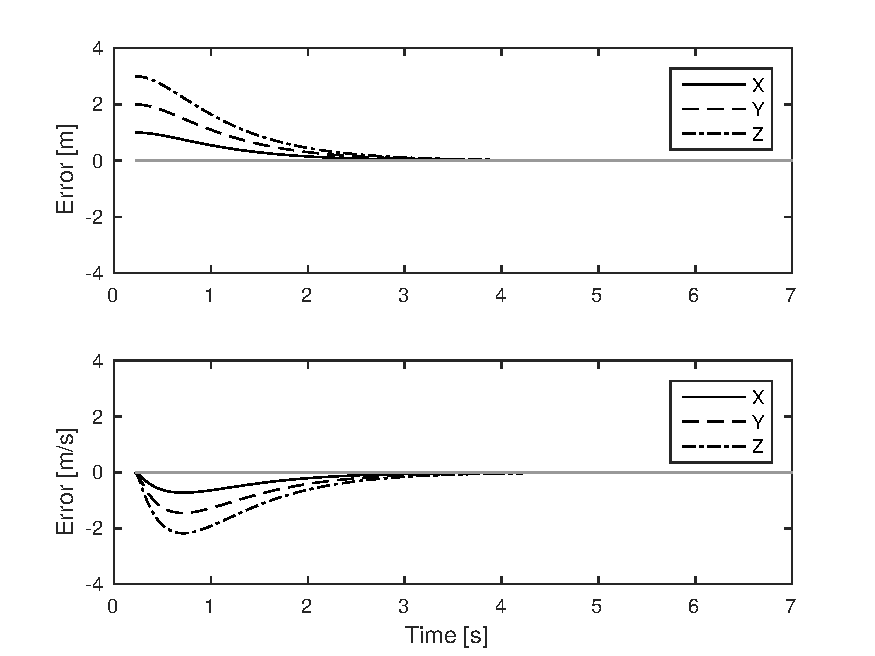
\includegraphics[width=0.8\linewidth]{error-p.pdf}
  \caption{Translational mode error convergence, from top to bottom: $e_x$ and $e_v$.}
  \label{fig:position_errors}
\end{figure}

On the attitude simulation, we start the vehicle at $(0\degree,0\degree,0\degree)$ and the reference is set as $(70\degree,-50\degree,30\degree)$ (both in $XYZ$ Euler angles). The results are shown in Figure~\ref{fig:attitude_errors}. Attitude convergence is approximately the same on all axis. As it depends only on the gains (equal for all axis) and the inertia of the vehicle (almost diagonal due to its symmetry), this result was also expectable.

\begin{figure}
  \centering
  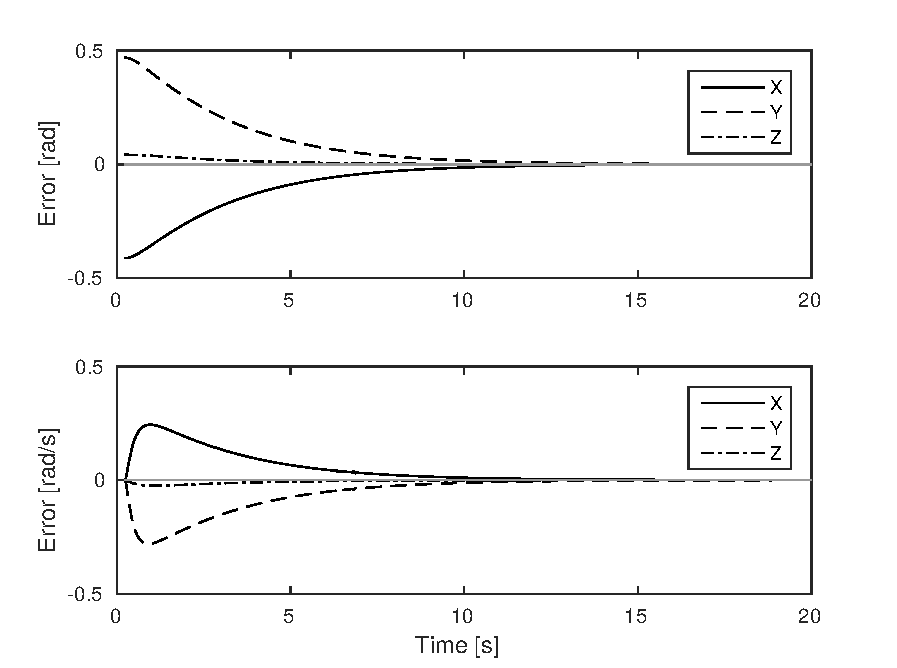
\includegraphics[width=0.8\linewidth]{error-a.pdf}
  \caption{Attitude mode error convergence, from top to bottom: $e_R$ and $e_\omega$.}
  \label{fig:attitude_errors}
\end{figure}


\subsection{Waypoint navigation and payload transportation}

To validate the joint position and attitude control, we used waypoint navigation: we created a virtual path composed by 6 waypoints, varying on both position and attitude. The trajectory followed by the vehicle is represented on \ref{fig:trajectory}. Plotted are both the X and Y axes of the body frame~$\mathcal{B}$ to represent its attitude. We retrieved the errors across the whole trajectory following, for both position and atitude. These are shown in Figure~\ref{fig:nav_errors}.

\begin{figure}
  \centering
  
\includegraphics[width=0.75\linewidth]{3d-trajectory.pdf}
  \caption{Trajectory followed by the robot without load. Plotted are X and Y axis of the inertia frame~$\mathcal{I}$.}
  \label{fig:trajectory}
\end{figure}

\begin{figure}
  \centering
  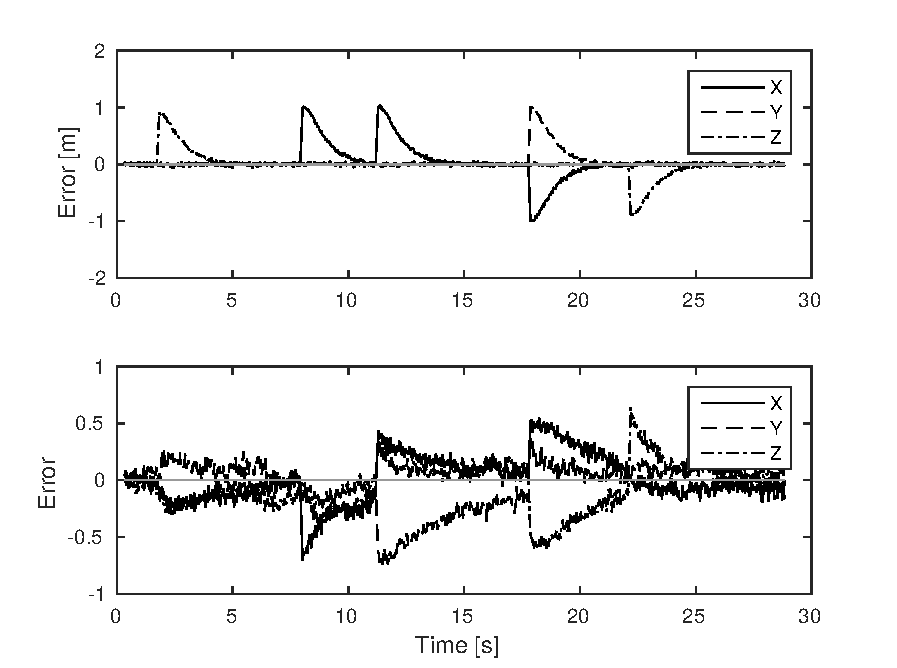
\includegraphics[width=0.8\linewidth]{robust-noload.pdf}
  \caption{Position (on top) and attitude (on bottom) errors along the no-load trajectory of Figure \ref{fig:trajectory}.}
  \label{fig:nav_errors}
\end{figure}

Then, we added a non-modeled payload to the system: a sphere with 6Kg of mass --- about the same mass of the vehicle. Even with such payload, the controller was able to converge to the required positions, though taking significantly more time. Shown on Figure~\ref{fig:loaded} are screenshots of the vehicle along its 3 waypoint trajectory: 1~meter up along Z and 1~meter right along Y. The position and attitude errors for this trajectory are plotted on Figure \ref{fig:nav_errors_load}

\begin{figure}
  \centering
  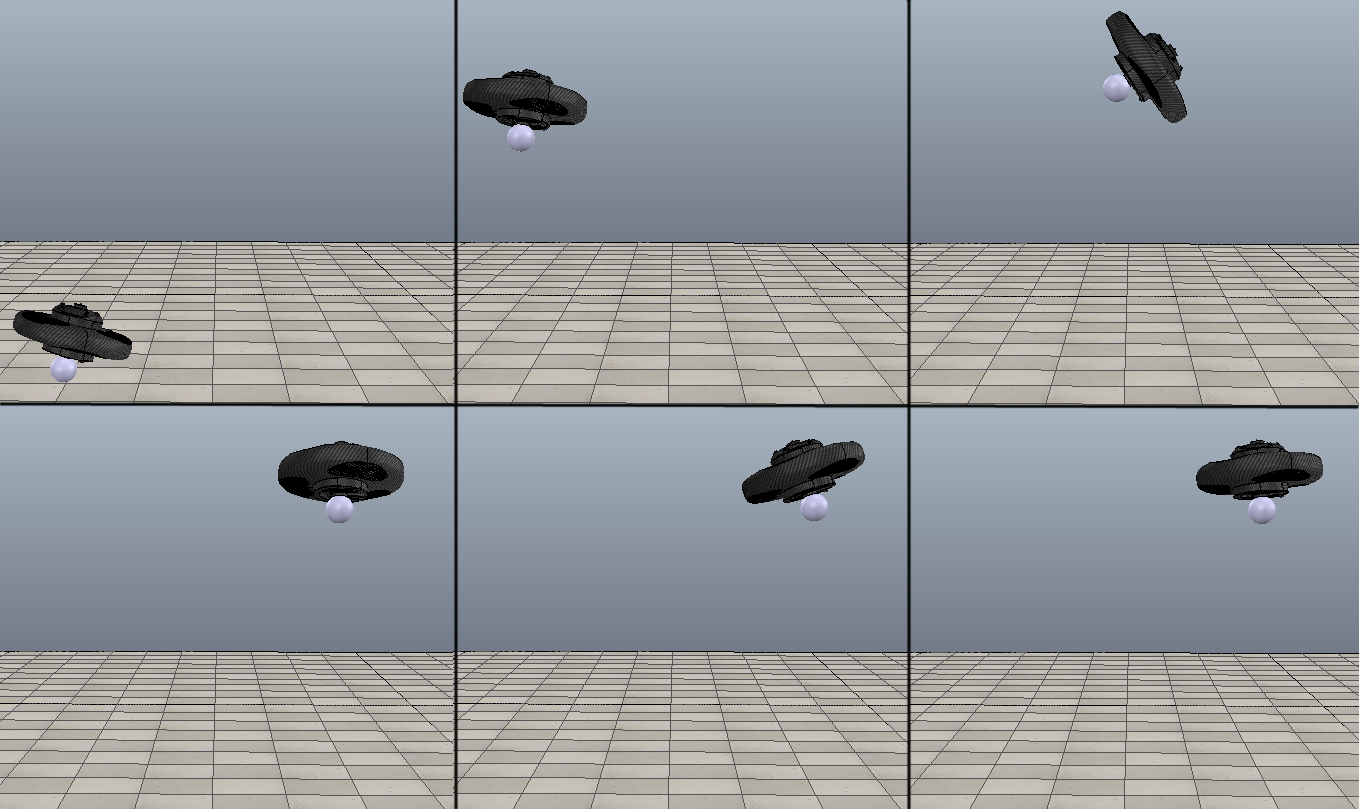
\includegraphics[width=0.75\linewidth]{snapshots.png}
  \caption{Trajectory followed by the robot with 6kg non-modeled load. Pictured are six positions of the robot along its trajectory.}
  \label{fig:loaded}
\end{figure}

\begin{figure}
  \centering
  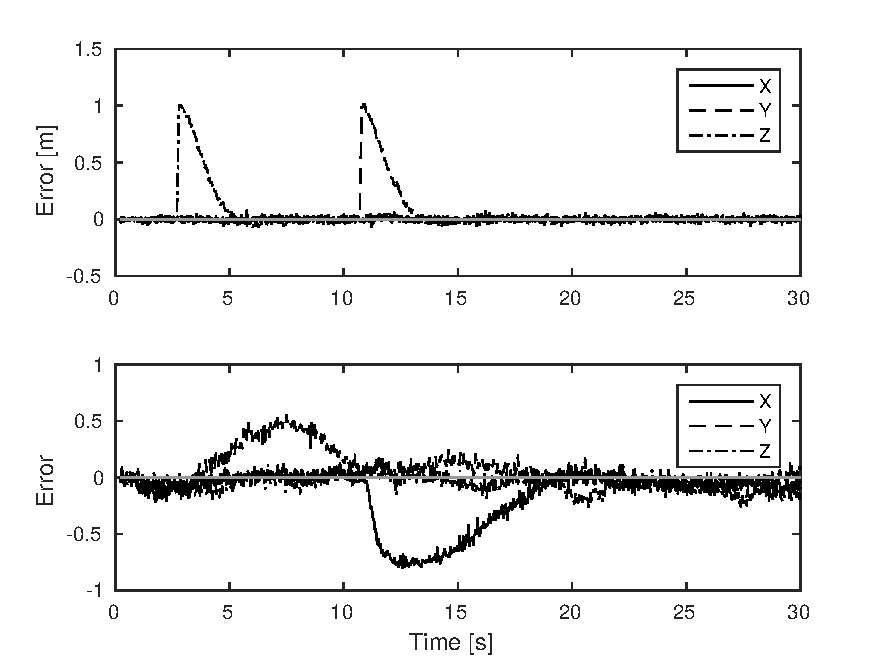
\includegraphics[width=0.8\linewidth]{robust-load.pdf}
  \caption{Position (on top) and attitude (on bottom) errors with non-modeled 6kg load along the trajectory of Figure \ref{fig:loaded}.}
  \label{fig:nav_errors_load}
\end{figure}





\subsection{Proof-of-concept tasks}
\label{sec:proof-concept-tasks}



\subsubsection{Debris Scavenging}
\label{sec:debis-scavenging}

One distinctive feature of microgravity environments is that objects
do not fall down to the floor when unreleased from one's hand. In a space
station environment, unattached objects, such as food debris, pens,
and even liquids, fly freely until coliding with something else, e.g.,
a wall. Therefore, astronats are required to manage manually such
objects, demanding additional cognitive effort. We propose here the automatic management of these objects by
Space CoBot. That is, we consider this robot to be able to detect and
track free flying debris, e.g., by the use of its camera array, and to
be equipped with a small vacuum cleaner capable of capturing and
storing them internally.

To provide a proof of concept for this task, we considered a small
object flying freely in an uncluttered environment. Since it
is free, the linear and angular velocities are constant. To
capture it we consider a three phase process: first, the Space CoBot
matches its trajectory at a distance $D_1$ of the object;
second, it approaches the object at a constant velocity with respect
to it until a threshold distance $D_2$ is achieved, where we consider it to be within reach of a small onboard vacuum
cleaner; finally, the object 
is sucked into the vehicle by it.

\begin{figure}
  \centering
  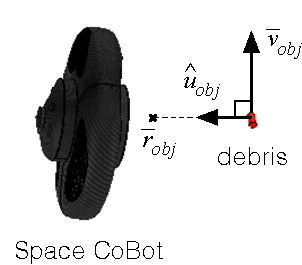
\includegraphics[width=0.6\linewidth]{debris_geometry.pdf}
  \caption{Geometry of the debris scavenging problem.}
  \label{fig:debris_geom}
\end{figure}

The geometry of the problem is shown in
Figure~\ref{fig:debris_geom}.
Let $\bar{x}_{obj}$ and $\bar{v}_{obj}$
be the object position and velocity. We define $\hat{u}_{obj}$ to be the
unit vector orthogonal to $\bar{v}_{obj}$ which
$\bar{x}_{obj}+\hat{u}_{obj}$ is closest to the Space CoBot
position. The position reference for tracking the object,
$\bar{r}_{obj}$, is defined along $\hat{u}_{obj}$, that is:
\begin{equation}
  \bar{r}_{obj} = \bar{x}_{obj} + d\,\hat{u}_{obj}
\end{equation}
In the first phase of the process, the Space CoBot matches its trajectory by
tracking $\bar{x}_d=\bar{r}_{obj}$ and $\bar{v}_d=\bar{v}_{obj}$ with
$d=D_1$. In the second, it
approaches the object at a constant velocity along $\hat{u}_{obj}$ by
decreasing $d$ at a constant rate from $D_1$ to $D_2$. Finally, when
the object is sufficiently close to the reference at $d=D_2$, it is sucked into the vehicle.

% CONSIDER SIMPLIFY THIS (RV):

% Let $\bar{x}_o$ be the object position and $\bar{v}_o$ its velocity. The first point is obtained by calculating a unit
% vector $\hat{u}$, orthogonal to the trajectory of the debree. This vector is given
% by
% \begin{equation}
%   \label{eq:vector_u}
%   \begin{aligned}
%     \vec{u} = \frac{ \bar{x} - \bar{x}_o - \left( \bar{x} - \bar{x}_o \right) \times \frac{\bar{v}_o}{|\bar{v}_o|} \cdot \frac{\bar{v}_o}{|\bar{v}_o|} }{|\bar{x} - \bar{x}_o - \left( \bar{x} - \bar{x}_o \right) \times \frac{\bar{v}_o}{|\bar{v}_o|} \cdot \frac{\bar{v}_o}{|\bar{v}_o|}|  }.
%   \end{aligned}
% \end{equation}
% Then,
% this vector is multiplied by $d$, thus giving the first setpoint,
% \begin{equation}
%   \label{eq:vector_u}
%   \begin{aligned}
%     \bar{x}_d &= \bar{x}_o+d \vec{u}, \\
%     \mathbf{R}_d &= \left[ \frac{\bar{v}_o}{|\bar{v}_o|} \ ; \ \vec{u}^T \times \frac{\bar{v}_o}{|\bar{v}_o|} \ ; \ \vec{u}^T    \right] ^T.
%   \end{aligned}
% \end{equation}
% When this
% objective is completed, the robot approaches the object along $\hat{u}$, while keeping
% its velocity. The results for the simulation, as well as an illustration of the whole task,
% is given on \ref{sec:sim-res}.



\begin{figure}
  \centering
  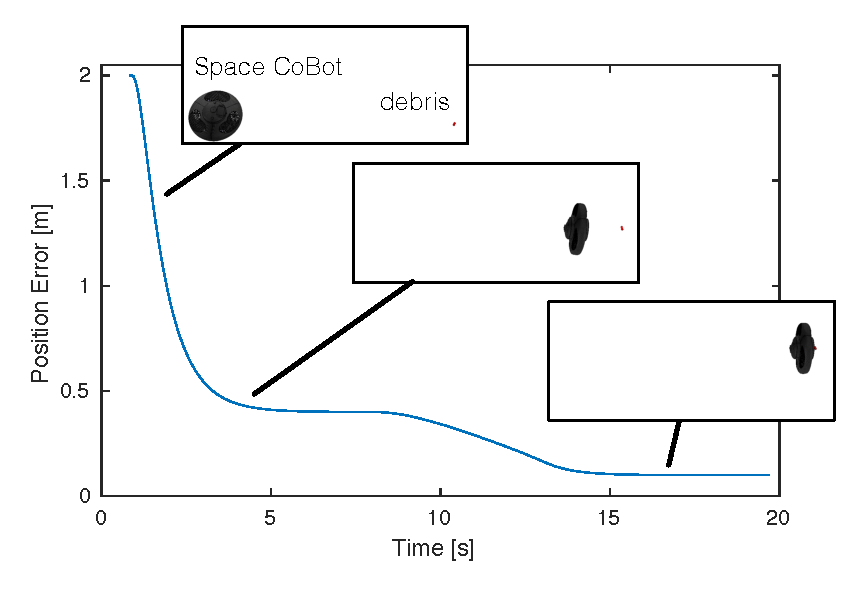
\includegraphics[width=\linewidth]{debris_comp.pdf}
  \caption{Simulation results for debris scavenging: distance from Space
    CoBot to the object position, along the three phases explained in
    the text.}
  \label{fig:debris-results}
\end{figure}

Figure~\ref{fig:debris-results} shows a simulation result of the
debris scavenging task. The target object is moving at a constant velocity of
0.03m/s along the $Y$ axis, while Space CoBot goes through the three
phases described above, also indicated in the figure. The distance between
the Space CoBot and the debris is plotted in this figure. Two plateaus
are visible: at $D_1=0.4m$, where Space CoBot matches the debris velocity,
and at $D_2=0.1m$, when we consider the object to be reachable by the robot.

% UPDATE THIS: For the first scene, Figure \ref{fig:debris-results} (a) illustrates the procedure described 
% on Section \ref{sec:debis-scavenging}. Plotted on Figure \ref{fig:debris-results} (b) is the norm of 
% the position error, relative to the object tracked. Note that this error
% does not converge to zero, as it is obtained by the difference between the
% the Center of Mass (CoM) of the space cobot and the CoM of the object and, therefore,
% a zero position error would mean that the object would be inside the robot. 

% On this image we can observe the 2 movement stages refered in  
% Section \ref{sec:debis-scavenging}. First, the robot stabilizes at 0.4 meters
% away of the debree and then it starts to approach the object linearly, until it
% is ready to be caught.

% \begin{figure*}
%   \def\gs{0.3}
%   \centering
%   \subfloat[]{\vbox{%
%       \def\gw{0.2}
%       \hbox{\fbox{
\includegraphics[width=\gw\linewidth]{figs/instace-1.png}}}
%       \hbox{\fbox{
\includegraphics[width=\gw\linewidth]{figs/instace-2.png}}}
%       \hbox{\fbox{
\includegraphics[width=\gw\linewidth]{figs/instace-3.png}}}
%       \hbox{\fbox{
\includegraphics[width=\gw\linewidth]{figs/instace-4.png}}}
%     }}
%   \hfil
%   \subfloat[]{
\includegraphics[height=\gs\linewidth, clip=true,
%       trim=4cm 10.3cm 4.5cm 8.8cm]{figs/debree.pdf}}
%   \caption{Debree Scavanging: (a)~trajectory performed by the Space CoBot;
%   to capture the debree; (b)~Norm of the Position Error in respect to the debree.}
%   \label{fig:debris-results}
% \end{figure*}

%, clip=true, trim=3.8cm 9.5cm 4.5cm 8.8cm



\subsubsection{Astronaut Stabilization}
\label{sec:astr-stab}

In microgravity, it is hard to keep the same position through time, as every little touch 
on indoor surfaces create a linear velocity and angular momentum on the astronauts body.
To overcome such problem, there are steel bars throughout the space station, which one
can grab and stabilize. Although this is a simple solution, there are situations in which 
these cannot be used, either because the user is performing a manual operation or because
these bars are out of range. 

Targeting these situations, we studied the use of a Space CoBot
attached to the back of the astronaut, like a backpack, that actively
uses its propulsion to reduce the astronaut velocity to zero, thus
stopping him from drifting. This is performed by using velocity
feedback only, that is, setting $\bar{v}_d=\bar{\omega}_d=0$ and
disabling the position/attitude feedback with $k_x=k_R=0$. By doing
so, the controller will counteract any non-zero motion of the
astronaut, both translational and rotational, while ignoring its
position.


% As we just want to stop the motion of the astronaut, the Proportional gained was turned off for 
% both experiments.

%On Section \ref{sec:sim-res} we provide the results for both tasks.



\begin{figure}
  \centering
  \subfloat[hit with a table]{%
    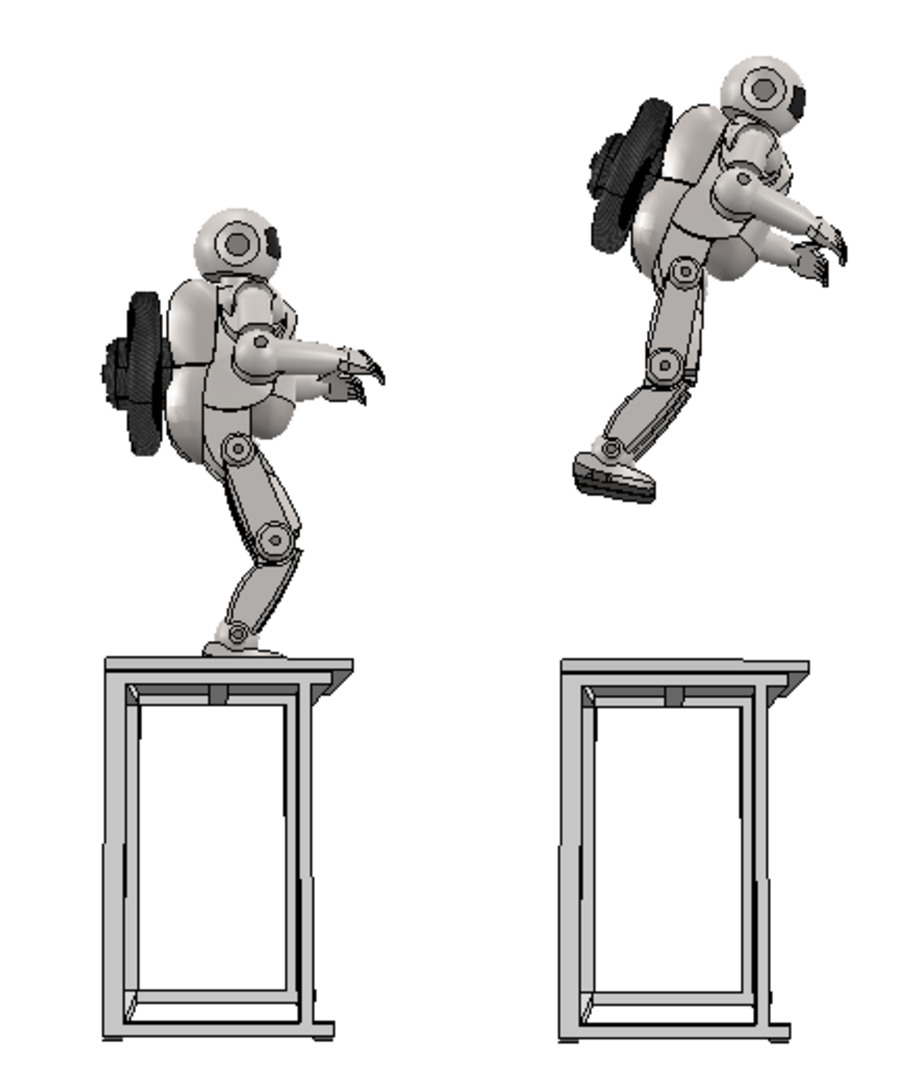
\includegraphics[width=0.4\linewidth]{astri_table.pdf}}
  \qquad
  \subfloat[hit with a wall]{%
    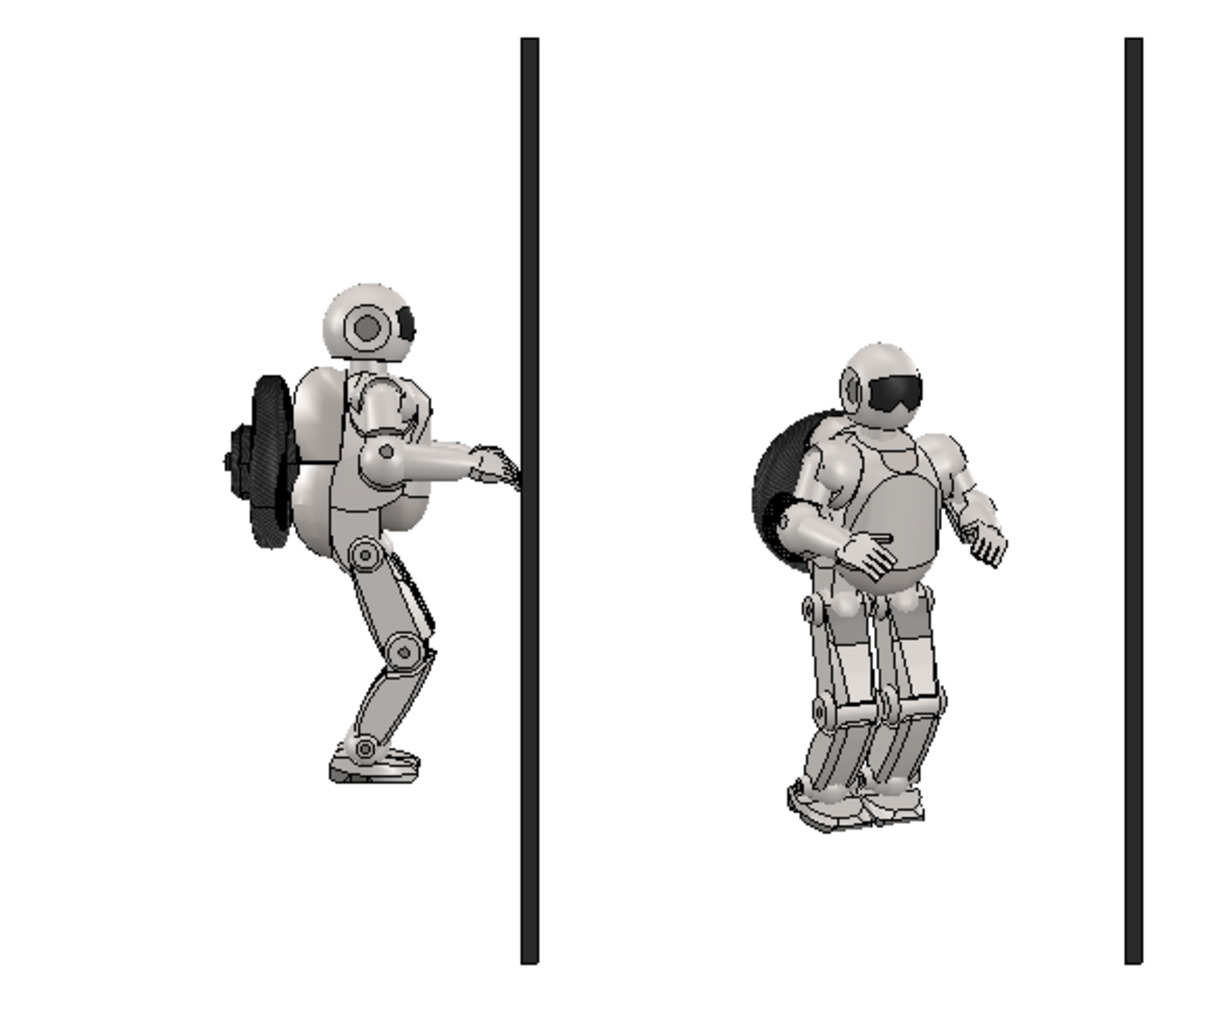
\includegraphics[width=0.5\linewidth]{astri_wall.pdf}}
  \caption{The two simulated situations for the astronaut
    stabilization task.}
  \label{fig:astri_table_wall}
\end{figure}

% \begin{figure}
% \centering
% \subfloat[]{%
%   \includegraphics[clip,width=0.5\columnwidth]{figs/table.pdf}%
% }
% \subfloat[]{%
%   \includegraphics[clip,width=0.9\columnwidth]{figs/astronaut-table.pdf}%
% }
% \caption{Astronaut Stabilization: (a)~Astronaut jumping on a fixed table;
% (b)~Norm of the velocity error along time, with and without stabilization, on
% the Space CoBot Center of Mass.}
% \label{fig:astronaut-table}
% \end{figure}

To simulate the astronaut stabilization task, we used the Astri
humanoid model, bundled with V-REP, to emulate the body dynamics of an
astronaut. Its total mass is 73Kg (12 times heavier than Space
CoBot). We tested two situations, illustrated in
Figure~\ref{fig:astri_table_wall}: in (a)~the astronaut stretches his
legs and hits the top of a table, while in (b)~the astronaut stretches his
arms and hits a vertical wall. In both cases, the hit provokes a
reaction momentum impelling the astronaut on the opposite direction to
the hit.

% The test is composed by two two experiments: on the first, we immobilize an astronaut
% --- represented in the simulation by the Asti robot model, with a
% total mass of 73kg, 12 times more than Space CoBot --- while
% it does a small jump; on the second we immobilize the individual when he pushes himself against 
% a wall.
 
% On the second scene, Figure \ref{fig:astronaut-table} (a) illustrates the jumping scene,
% while Figure \ref{fig:astronaut-table} (b), shows the results of jumping
% with and without active stabilization, through the plots of the norm for
% the velocity error.

For each one of these situations we compared the trajectories of Space
CoBot, always attached to the astronaut, with and without the
controller. Plots of the translational velocity norm of the robot CoM
are shown in Figure~\ref{fig:table-wall-plot}. It is visible in both
cases that the controller successfully stabilizes motion in about 4
seconds. The oscillatory behavior when the controller is disabled
corresponds to the velocity, with respect to the inertial frame, of
the robot CoM ``orbiting'' the resultant CoM of astronaut+robot, while
it drifts away from the contact point.

\begin{figure}
  \centering
  \subfloat[hit with a table]{%
    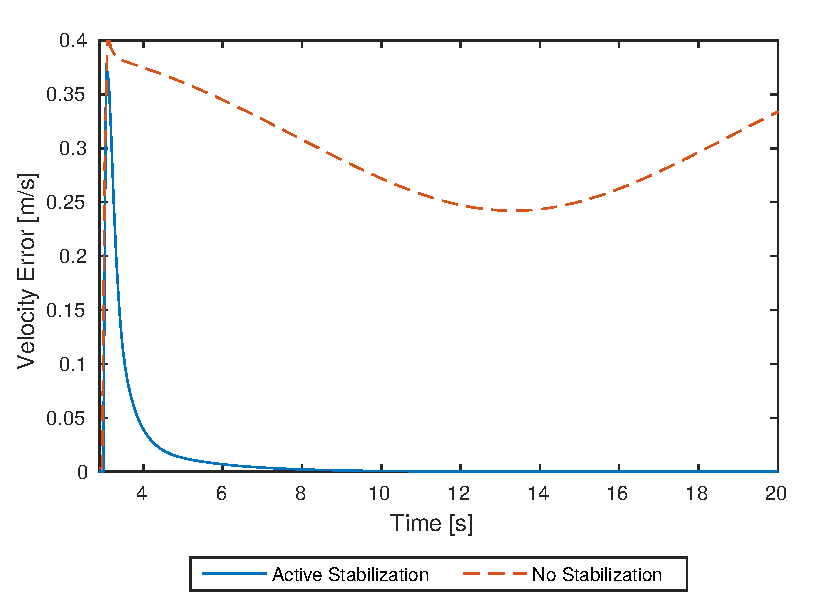
\includegraphics[width=\linewidth]{plot_table.pdf}} \\
  \subfloat[hit with a wall]{%
    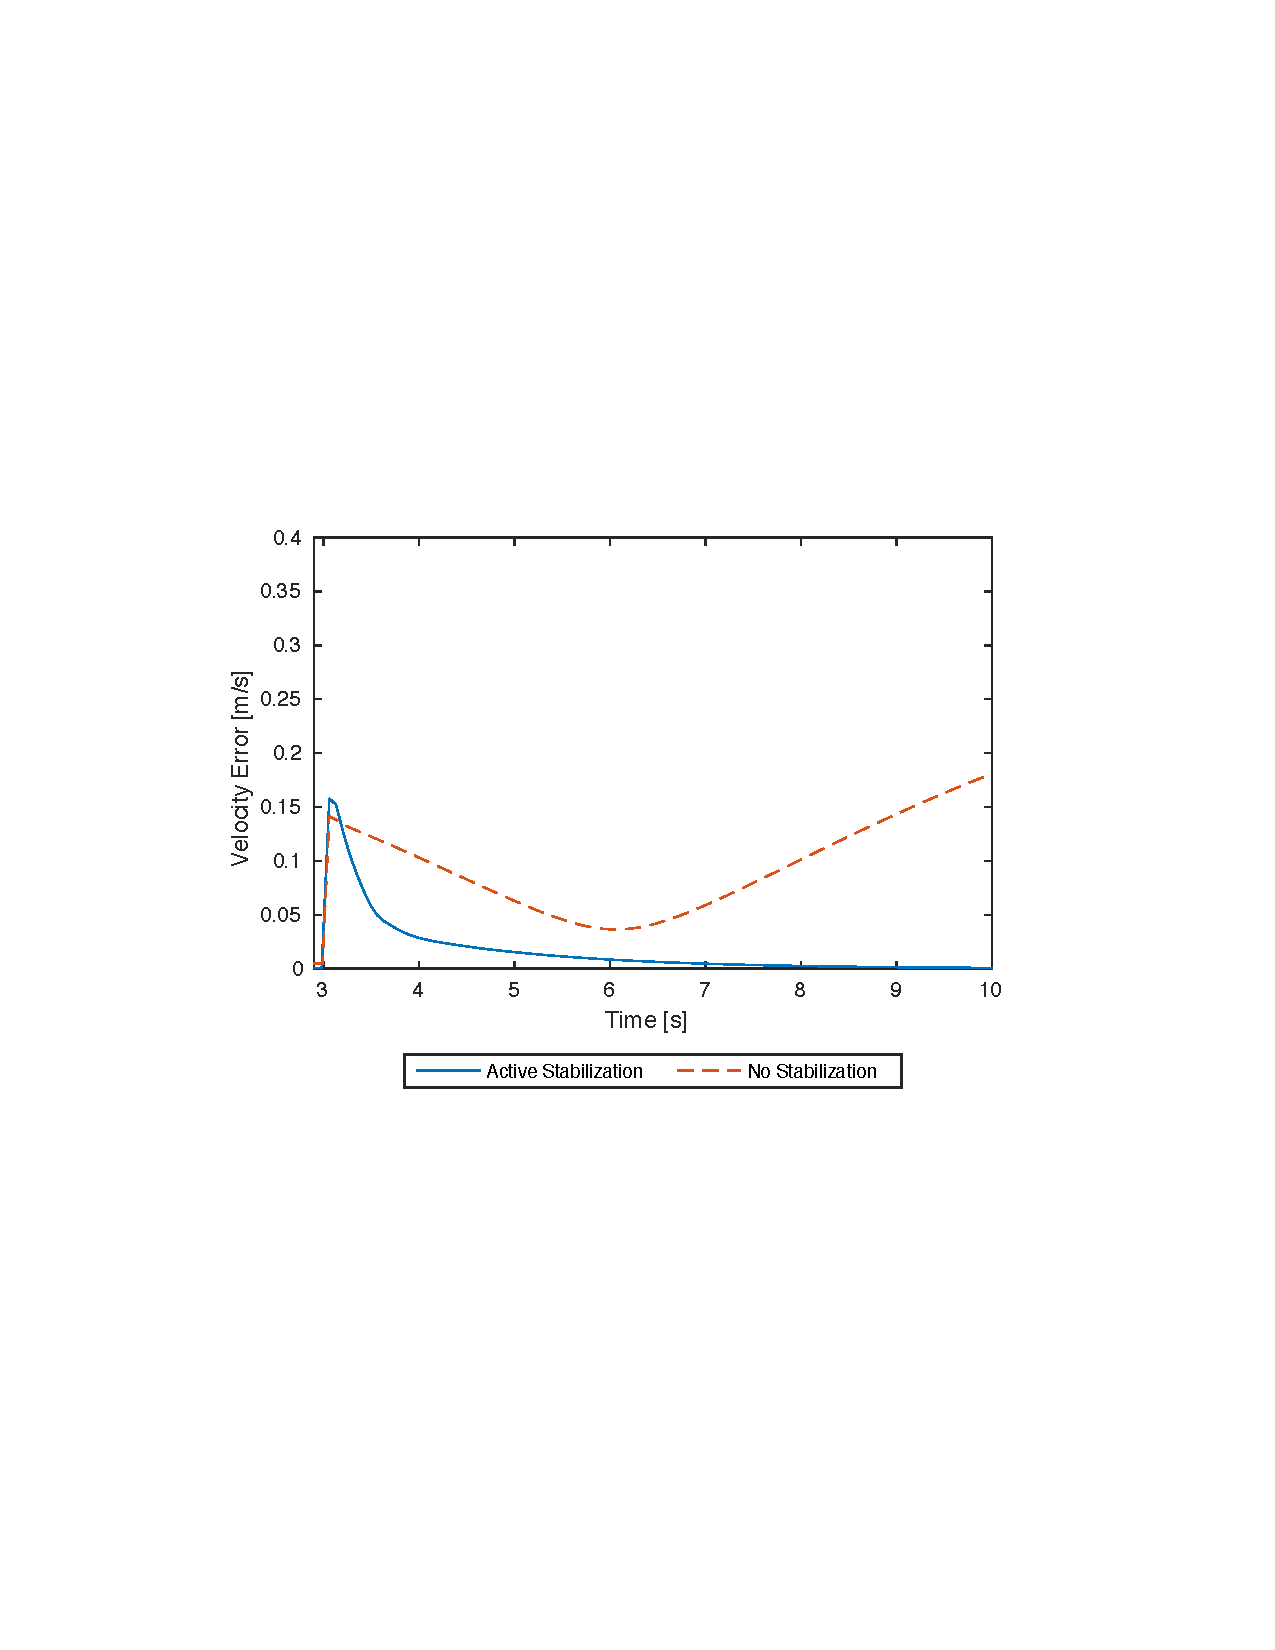
\includegraphics[width=\linewidth]{plot_wall.pdf}}
  \caption{Norm of the linear velocity of Space CoBot, with and
    without motion stabilization, for the two situations described in
    the text.}
  \label{fig:table-wall-plot}
\end{figure}

% When activated, the Space CoBot can successfully stabilize an astronaut in about
% 3 seconds, even though it has 12 times less the mass of astronaut model.
% Note that the velocity norm error presented is expressed for the robot CoM, and for the 
% CoM of the joint masses. Therefore, as the astronaut spins, the velocity without
% stabilization oscillates due to the momentum imposed by the force of the jumping movement.




% TODO: move this somewhere else
All of the simulations discussed in this section were compiled into a
video available here: \\
\centerline{\url{https://youtu.be/TQqRAMBv3-M}}






\section{Related work}
\label{sec:related-work}

Early experiments with free flyers robots in space were performed with
the AERCam “Sprint” platform in the late 1990’s on the Space Shuttle
payload bay, for extra-vehicular remote inspection. Efforts to a
smaller version began in early 2000’s, with the Mini
AERCam~\cite{wagenknecht03}, but it was never deployed in space.

The SPHERES are small free-flyer microgravity robots~\cite{miller00},
developed by NASA and deployed at ISS in 2006. There are 3 of them
currently in operation, mostly hosting scientific experiments in
various domains, such as in computer vision~\cite{tweddle12},
formation flight~\cite{eslinger13}, and fluid
mechanics~\cite{burke10}. These robots are fully actuated, propelled
by 12 nozzles expelling CO2 in a controlled fashion. The internal CO2
tank limits operation from a 20 seconds to 30 minutes range duration.

More recently, NASA has been developing the Astrobee free-flyers,
succeeding SPHERES in its goals, while adding a broad range of
functionalities~\cite{bualat15}. Two of these platforms are planned to be deployed on
the ISS by 2018. The Astrobee propulsion is based on servo controlled
nozzles expelling low pressure air, obtained from two counter rotating
centrifugal pumps and stored in a plenum. It is equipped with multiple
cameras, RGB and depth, one of them being used for vision-based
navigation~\cite{coltin16}. It includes two bays, one at the bottom to hosting
scientific experiments, and one at the top where a 2 DoF perching arm
will be mounted. This arm was designed for Astrobee to attach to the
hand rails on the ISS, for power saving while not being used. In
addition, a docking station is being designed for charging. Its HRI is
based on stripes of colored LEDs conveying information to the human
operators.

CIMON (Crew Interactive Mobile CompanioN) is an European free-flyer
being developed by DLR, Airbus DS, IBM, and the Ludwig Maximilian
University in Munich, designed to be an autonomous assistant system
for astronauts in the ISS. It is also based on an air propulsion
system and vision based navigation.  Based on the well-known IBM's
Watson platform, it aims at providing assistance through dialogue in
natural language. This platform targets three tasks: (1)~crew support
in their daily routines, (2)~video documentation, and (3)~trainning of
astronauts for specific skills. Scarce information about this platform
has been disclosed. It is expected to be launched to the ISS in 2018.

The Japanese JAXA has also been developing a free-flyer for the ISS,
called Internall Ball Camera (Int-Ball), recently deployed in the
ISS. Motion is based on a combination of 12 propulsion fans together
with reaction wheels, and its navigation is vision based. Its purpose
is to be a high resolution flying camera with image stabilization.

% Both SPHERES and Astrobee were validated on ground using two systems:
% an air-bearing support on a flat table, for 2D motion, and an active
% gimbal for full 6D motion. Preparation of these platforms to be
% actually deployed in space is a lengthy and thorough process, lasting
% a few years.

% PLACE TABLE HERE

% Besides these, another project with a little different perspective but
% also employing human interaction with technology onboard the ISS was
% developed by the Irish company Space Synapse, managed by the artist
% Anna Hill, which aims at sharing the human experience of space travel
% with everyone on Earth. To this purpose the company offers the
% Symbiotic Sphere~\cite{hill04} which is designed to gather any
% sensorial data (images, video, sounds, biomedical information,
% housekeeping and other data flow) from within the ISS in order to
% transmit it to the ground. This metallic sphere is designed to
% free-float on microgravity, communicate wirelessly and to interact
% with the astronauts by projecting images onto astronauts’ hands. The
% sphere is also able to anchor and recharge in a docking device that
% pulsates according to information flow.

% add CIMON and Japanese thingy

\section{Conclusions and future work}
\label{sec:concl-future-work}



\section*{References}

\bibliography{biblio}

\end{document}